
%\def\anon{1} %% set to 1 for anonymous submissions, hides acknowledgements and author names
\def\full{1} %% set to 0 for springer proceedings


\ifnum\full=1
\documentclass[11pt]{llncs}


\addtolength{\parskip}{1pt}
\else
\documentclass[10pt, runningheads]{llncs}
\usepackage{times}
\fi




\usepackage{makeidx}
\usepackage[dvips]{graphicx}
\usepackage{graphicx}

\usepackage{comment}

\usepackage{listings}
\usepackage[mathscr]{eucal}
\usepackage{bm}
\usepackage{array}
\usepackage{url}
\usepackage{calc}
\usepackage{float}
\usepackage{latexsym}
\usepackage{rotating}
\DeclareGraphicsExtensions{.eps,.jpg,.png,.pdf}
\usepackage[usenames, dvipsnames]{xcolor}
\usepackage[sort,nocompress]{cite}
\usepackage{colortbl}
\usepackage{multirow}
\usepackage{lscape}
\usepackage{amsmath}
\let\proof\relax
\let\endproof\relax
\usepackage{amsthm,amsfonts,amssymb}
\usepackage{hyperref}
\usepackage{pdflscape}


%\usepackage{natbib}

\def\rmdefault{ptm}



\usepackage{setspace}
\usepackage{color}
\ifnum\full=1
\usepackage[margin=0.9in]{geometry}
\usepackage{fullpage}

\setlength{\parskip}{0cm}

%\setstretch{1.03}
%\addtolength{\parskip}{1pt}
\setcounter{page}{0}
\renewcommand{\tabcolsep}{5pt}
\else
\renewcommand{\tabcolsep}{0pt}
\fi

\renewcommand{\arraystretch}{1.2}

\hyphenpenalty=5000
\tolerance=1000




%\ifnum\full=1
%\usepackage{natbib}
%\bibliographystyle{alpha}
%\setlength{\bibsep}{0pt}
%\renewcommand{\bibsection}{\section*{References}\small}
%\else
%\usepackage[numbers]{natbib}
%\bibliographystyle{splncs04}
%\fi



\DeclareMathOperator{\Exp}{E}
\DeclareMathOperator{\Var}{Var}
\DeclareMathOperator{\poly}{poly}
\DeclareMathOperator{\Supp}{Supp}

\usepackage{enumitem}


\usepackage{tikz}
\usetikzlibrary{arrows,shapes}
\usetikzlibrary{plotmarks}


%notes

%\definecolor{myorange}{rgb}{0.99,0.6,0.25}
%\newcommand{\pmnote}[1]{\colorbox{myorange}{\parbox{0.9\linewidth}{[{\footnotesize {\bf PM:} { {#1}}}]}}}


\definecolor{mycolor}{rgb}{0.75,0.95,0.05}
\newcommand{\pmnote}[1]{\colorbox{mycolor}{\parbox{0.9\linewidth}{[{\footnotesize {\bf PM:} { {#1}}}]}}}

\definecolor{color2}{rgb}{0.95,0.9,0.2}
\newcommand{\lbnote}[1]{\colorbox{color2}{\parbox{0.9\linewidth}{[{\footnotesize {\bf LB:} { {#1}}}]}}}


%% Sets

\newcommand{\Z}{\mathbb{Z}}
\newcommand{\N}{\mathbb{N}}
\newcommand{\R}{\mathbb{R}}
\newcommand{\F}{\mathbb{F}}
\newcommand{\Znm}{\mathbb{Z}_q^{n \times m}}

%matrices
\newcommand{\matzero}{\mathbf{0}}
\newcommand{\matA}{\mathbf{A}}
\newcommand{\matB}{\mathbf{B}}
\newcommand{\matC}{\mathbf{C}}
\newcommand{\matE}{\mathbf{E}}
\newcommand{\matF}{\mathbf{F}}
\newcommand{\matG}{\mathbf{G}}
\newcommand{\matI}{\mathbf{I}}
\newcommand{\matM}{\mathbf{M}}
\newcommand{\matP}{\mathbf{P}}
\newcommand{\matR}{\mathbf{R}}
\newcommand{\matS}{\mathbf{S}}
\newcommand{\matT}{\mathbf{T}}
\newcommand{\matU}{\mathbf{U}}
\newcommand{\matV}{\mathbf{V}}
\newcommand{\matW}{\mathbf{W}}
\newcommand{\matX}{\mathbf{X}}
\newcommand{\matY}{\mathbf{Y}}
\newcommand{\matZ}{\mathbf{Z}}


%vectors
\newcommand{\veca}{\mathbf{a}}
\newcommand{\vecb}{\mathbf{b}}
\newcommand{\vecc}{\mathbf{c}}
\newcommand{\vecd}{\mathbf{d}}
\newcommand{\vece}{\mathbf{e}}
\newcommand{\veci}{\mathbf{i}}
\newcommand{\vecj}{\mathbf{j}}
\newcommand{\veck}{\mathbf{k}}
\newcommand{\vecl}{\mathbf{l}}
\newcommand{\vecm}{\mathbf{m}}
\newcommand{\vecp}{\mathbf{p}}
\newcommand{\vecr}{\mathbf{r}}
\newcommand{\vecs}{\mathbf{s}}
\newcommand{\vecv}{\mathbf{v}}
\newcommand{\vecw}{\mathbf{w}}
\newcommand{\vecu}{\mathbf{u}}
\newcommand{\vecx}{\mathbf{x}}
\newcommand{\vecy}{\mathbf{y}}
\newcommand{\vecz}{\mathbf{z}}





%FiLIP notations

\newcommand{\FLIP}{\textsf{FLIP}}
\newcommand{\IFPl}{\text{Improved Filter Permutator} }
\newcommand{\IFPs}{\text{IFP} }

\newcommand{\FiLIP}{\textsf{FiLIP}}
\newcommand{\FiLIPDSM}{\mathsf{FiLIP}_{\mathsf{DSM}}}
\newcommand{\FiLIPXMAJ}{\mathsf{FiLIP}_{\mathsf{XMAJ}}}

%Boolean functions

\newcommand{\Bfn}[1]{\mathcal{B}_{#1}}
\newcommand{\BN}{\mathcal{B}_n}
\newcommand{\Bn}[1]{\mathcal{B}_{#1}}
\newcommand{\Bnstar}[1]{\mathcal{B}_{#1}^*}

\newcommand{\Bvad}[3]{\mathcal{B}({#1},{#2},{#3})}


\newcommand{\AI}{\mathsf{AI}}
\newcommand{\AIk}[1]{\mathsf{AI}_{#1}}
\newcommand{\AN}{\mathsf{AN}}
%\newcommand{\difAN}[1]{\Delta_{\mathsf{AN}}(#1)}
%\newcommand{\DAN}{\mathsf{d}\mathsf{AN}}
%\newcommand{\Sd}{\mathsf{S}_\mathsf{d}}
\newcommand{\SD}{\mathsf{SD}}
\newcommand{\FAI}{\mathsf{FAI}}
\newcommand{\NL}{\mathsf{NL}}
\newcommand{\NLk}[1]{\mathsf{NL}_{#1}}
%\newcommand{\NLd}{\mathsf{NL_d}}
\newcommand{\res}{\mathsf{res}}
\newcommand{\bal}{\mathsf{bal}}
\newcommand{\gnlk}{\mathsf{GWNL}}


\newcommand{\DS}[1]{\mathsf{DS}(#1)}
\newcommand{\DSR}[2]{\mathsf{DS}^{#2}(#1)}
%\newcommand{\matAI}[3]{\mathbf{A}_{#2,#3}(#1)}

\newcommand{\WPB}[1]{\mathcal{WPB}_{#1}}
\newcommand{\WAPB}[1]{\mathcal{WAPB}_{#1}}
\newcommand{\SWAPB}[1]{\mathcal{SWAPB}_{#1}}
\newcommand{\SYM}[1]{\mathcal{SYM}_{#1}}
%for affine weightwise: degree and number of variables
\newcommand{\WD}[2]{\mathcal{WD}^{#1}_{#2}}
\newcommand{\Ekn}[2]{\mathsf{E}_{#1,#2}}
\newcommand{\Code}[2]{\mathsf{P}_{#1,#2}}
\newcommand{\mdist}[2]{\mathsf{d}_{#1,#2}}


\newcommand{\mnlk}[2]{\mu_{#1,#2}}
\newcommand{\Mnlk}[2]{\mathsf{M}_{#1,#2}}
\newcommand{\mnl}[1]{\mu_{#1}}
\newcommand{\Mnl}[1]{\mathsf{M}_{#1}}

\newcommand{\DistWkn}[2]{\mathfrak{W}_{#1,#2}}
\newcommand{\DistWn}[1]{\mathfrak{W}_{#1}}
\newcommand{\Dkn}[2]{\mathfrak{D}_{#1,#2}}
\newcommand{\Dn}[1]{\mathfrak{D}_{#1}}

\newcommand{\kraw}[3]{\mathsf{K}_{#1}(#2,#3)}
\newcommand{\phikn}[2]{\varphi_{#1,#2}}

\newcommand{\const}[2]{g_{#1,#2}}
\newcommand{\setn}[1]{S_{#1}}
\newcommand{\symsetsmall}[1]{A_{#1}}
\newcommand{\symset}[2]{B_{#1,#2}}


%usual notations
\newcommand{\supp}{\mathsf{supp}}
\newcommand{\suppk}[1]{\mathsf{supp}_{#1}}
\newcommand{\w}{\mathsf{w_H}}
\newcommand{\hd}{\mathsf{d_H}}
\newcommand{\degg}{\mathsf{deg}}
\newcommand{\Span}{\mathsf{Span}}
\newcommand{\rank}{\mathsf{rank}}
%Walsh transform
\newcommand{\wt}[1]{W_{#1}} 
\newcommand{\Wsupp}[1]{\mathsf{Wsupp}_{#1}} 
%restricted Walsh transform W_k,a (f)
\newcommand{\wtk}[2]{\mathcal{W}_{#1,#2}} 

%S-equivalent classes
\newcommand{\sclass}[1]{\mathcal{S}(#1)}


\newcommand{\set}[1]{\left\{#1\right\}}
\newcommand{\mAN}[1]{\mathsf{d}_{#1}}


%gates
\newcommand{\AND}{\textsf{AND}}
\newcommand{\XOR}{\textsf{XOR}}
\newcommand{\MUX}{\textsf{MUX}}


%families of functions
\newcommand{\MAJ}{\textsf{MAJ}}
\newcommand{\DSM}{\textsf{DSM}}
\newcommand{\XORTHR}{\textsf{XOR-THR}}
\newcommand{\XORMAJ}{\textsf{XOR-MAJ}}

\newcommand{\xorlk}[2]{{\mathsf{XOR}}_{#1}  \mathsf{M}_{#2}} 
\newcommand{\xormaj}[2]{{\mathsf{XOR}}_{#1}  \mathsf{MAJ}_{#2}} 
%\newcommand{\xorthr}[3]{{\mathsf{XOR}}_{#1}  \mathsf{T}_{{#2},{#3}}} 
\newcommand{\xorthr}[3]{{\mathsf{XOR}}_{#1}+\mathsf{T}_{{#2},{#3}}}
\newcommand{\tri}[1]{{T}_{#1}}
\newcommand{\thr}[2]{\mathsf{T}_{{#1},{#2}}}
\newcommand{\xor}[1]{\mathsf{XOR}_{#1}}
\newcommand{\maj}[1]{\mathsf{MAJ}_{#1}}


\newcommand{\nbf}[1]{\mathsf{C}_{#1}}
\newcommand{\nbfodd}[2]{\mathsf{A}_{#1,#2}}
\newcommand{\nbfeven}[2]{\mathsf{B}_{#1,#2}}

%direct sum vector and simplified value vector
\newcommand{\dsv}[1]{\mathbf{m}_{#1}}
\newcommand{\svv}[1]{\mathbf{s}_{#1}}



\newtheorem{Prop}{Property}
\newtheorem{Cons}{Construction}


% For algorithms
\usepackage{algorithm,algpseudocode}

\renewcommand{\algorithmicrequire}{\textbf{Input:}}
\renewcommand{\algorithmicensure}{\textbf{Output:}}
% \renewcommand{\ALG@name}{Construction}
\newenvironment{constr}[1][htb]{%
\floatname{algorithm}{Construction}% Update algorithm name
   \begin{algorithm}[#1]%
  }{\end{algorithm}}
 
\algnewcommand\algorithmicparfor{\textbf{par-for}}
\algdef{S}[FOR]{ParFor}[1]{\algorithmicparfor\ #1\ \algorithmicdo}
 
%latin

\newcommand{\ie}{\textit{i.e.} }
\newcommand{\eg}{\textit{e.g.} }
\newcommand{\ea}{\textit{et al.} }




\usepackage{placeins}

\begin{document}
	\title{Title}

	
	\titlerunning{title}
	
	
%\if\anon=1	
	\author{
		\mbox{Luca Bonnamino, Pierrick M\'eaux}%\inst{1}
	}
	
	\authorrunning{L. Bonnamino, P. M\'eaux}
	
	\institute{
	Luxembourg university, Luxembourg\\
		\email{pierrick.meaux@uni.lu}		
	}
	
%\fi
	
	
	
	%----------------------------------------------------------------
	\maketitle


%\institute{
%	University of Luxembourg, Luxembourg\\
%	\email{pierrick.meaux@uni.lu}		
%}	
	
	\begin{abstract}

		
\keywords{Boolean functions, Weightwise perfectly balanced functions, Cryptographic criteria.}		
		
	\end{abstract}



\section{Introduction}

\pmnote{recall here the main idea of finding AI and rank of Reed Muller code, maybe re-read the explanation in "Extreme algebraic attacks"}

\lbnote{example}



\section{Preliminaries}\label{sec:prelim}


For readability, we use the notation $+$ instead of 
$\oplus$ to denote the addition in $\F_2$, and $\sum$ instead of $\bigoplus$. 
In addition to classic notations, we denote by $ [a,b] $ the subset of all integers between $a$ and $b$: $\{a, a+1, \ldots,b\}$. 
For a vector $v\in \F_2^n$ we use $\w(v)$ to denote its Hamming weight $\w(v)=|\{ i \in [1,n] \, | \, v_i=1 \}|$. 
For two vectors $v$ and $w$ in $\F_2^n$ we denote by $\hd(v,w)$ the Hamming distance between $v$ and $w$, that is, $\hd(v,w)=\w(v+w)$. 
For two functions $f$ and $g$ we denote by $\hd(f,g)$ the Hamming distance between their vectors of values.

\subsection{Ordering relations on \texorpdfstring{$\mathbb{F}_2^n$}{F\_2^n}}
Let $n\in \N^*$
\begin{definition}[Tot-WOrd relation on a field]\label{def:orderingOnK}
	Let $K$ be a field. We define a Tot-WOrd ordering relation $<_{Ord_K}$ as a total and well-ordering relation on $K$, that is
	\begin{itemize}
		\item $<_{Ord_K}$ is a total ordering in $K^{n}$
		\item Let $\alpha, \beta, \gamma \in K$, if $\beta <_{Ord_K} \alpha$ then $\beta + \gamma <_{Ord_k} \alpha + \gamma$
		\item Any non-empty subset of $K$, has a smaller element under $<_{Ord_K}$: if $S \subset K \neq \emptyset$, then there is a $\alpha$ such that $\alpha <_{Ord_K} \beta$ for every $\beta \in S$ such that $\beta \neq \alpha$. 
	\end{itemize}
\end{definition}

\begin{definition}[Tot-WOrd relation on $\F_2^n$]\label{def:OrderingOnF2n}
	a Tot-WOrd ordering relation $ord$ on $\F_2^n$ is a total ordering $<_{ord_{\F_n^2}}$ between elements of $\F_2^n$.\\
	Since in the document we only consider total, well ordered orderings, we omit the Tot-WOrd prefix in the ordering name: we call Tot-WOrd ordering relation on $\mathbb{F}_2^n$ as an \textit{ordering relation} on $\mathbb{F}_2^n$. 
\end{definition}

Two ordering relations in $\mathbb{F}_2^n$ are used in this project: the \textit{lexicographic} and the \textit{graded lex} order.

\begin{definition}[Lexicographic order]
	Let $\alpha = (\alpha_n, \alpha_{n-1}, \cdots, \alpha_1) \in \mathbb{F}_2^n$ and $\beta = (\beta_n, \beta_{n-1}, \cdots, \beta_1) \in \mathbb{F}_2^n$.\\
	The \textit{lexicographic} ordering relation on $\mathbb{F}_2^n$ is a ordering relation $<_{lex}$ on $\mathbb{F}_2^n$ such that $\beta <_{lex} \alpha$ if the leftmost nonzero entry of the vector difference $\hat{\alpha}-\hat{\beta}$ is positive.
\end{definition}

\begin{definition}[Graded Lex order]
	Let $\alpha = (\alpha_n, \alpha_{n-1}, \cdots, \alpha_1) \in \mathbb{F}_2^n$ and $\beta = (\beta_n, \beta_{n-1}, \cdots, \beta_1) \in \mathbb{F}_2^n$.\\
	The \textit{graded lex} ordering relation on $\mathbb{F}_2^n$ is a ordering relation $<_{grlex}$ on $\mathbb{F}_2^n$ such that
	We say $\beta <_{grlex} \alpha$ if
	\begin{align*}
	w_H(\beta) < w_H(\alpha) \mbox{ or }  \left(w_H(\beta) = w_H(\alpha) \mbox{ and } \beta <_{lex} \alpha\right)
	\end{align*}
\end{definition}

\begin{definition}[Ordering relation on a set]
	We define the function 
	\begin{align*}
	Ord: S = \{s_1, s_2, \cdots, s_{|S|}\} \subseteq \mathbb{F}_2^n \mapsto \left(s_{\sigma(s)}\right)_{s\in S} = \left(s_{\sigma(1)}, s_{\sigma(2)}, \cdots, s_{\sigma(|S|)}\right)
	\end{align*}
	where $\sigma$ is the permutation assigning the index of an element of the ordered vector by the ordering $Ord$, to the index of the element in the original set $S$, i.e. $\sigma$ is such that 
	\begin{align*}
	s_{\sigma(i)} <_{ord} s_{\sigma(j)} \mbox{ for } i<j
	\end{align*}
\end{definition}

\begin{definition}[Lexicographical order relation on a set]
	We define the function $Lex: S = \{s_1, s_2, \cdots, s_{|S|}\} \subseteq \mathbb{F}_2^n \mapsto \left(s_{\sigma(s)}\right)_{s\in S} = \left(s_{\sigma(1)}, s_{\sigma(2)}, \cdots, s_{\sigma(|S|)}\right)$, where $\sigma$ is such that $s_{\sigma(i)} \leq_{lex} s_{\sigma(j)}$ for $i<j$:
\end{definition}

\begin{definition}[Graded Lex order relation on a set]
	We define the function $GrLex: S = \{s_1, s_2, \cdots, s_{|S|}\} \subseteq \mathbb{F}_2^n \mapsto \left(s_{\sigma(s)}\right)_{s\in S} = \left(s_{\sigma(1)}, s_{\sigma(2)}, \cdots, s_{\sigma(|S|)}\right)$, where $\sigma$ is such that $s_{\sigma(i)} <_{grlex} s_{\sigma(j)}$ for $i<j$:
\end{definition}

\subsection{Boolean functions, cryptographic criteria, and weightwise properties}
In this section, we recall fundamental concepts concerning Boolean functions and their weightwise properties, which are utilized throughout this article. For a more comprehensive introduction to Boolean functions and their cryptographic parameters, we recommend consulting the book by Carlet~\cite{Carlet20},
%consulting for instance the book by Carlet~\cite{Carlet20}, 
and for insights into weightwise properties—also known as properties on the slices—the article by~\cite{TOSC:CarMeaRot17}.
We denote by $\Ekn{k}{n}$ the set $\{x\in \F_2^n \, | \, \w(x)=k \}$ for $k \in [0,n]$, referring to it as a slice of the Boolean hypercube (of dimension $n$). 
Consequently, the Boolean hypercube is divided into $n+1$ slices, where the elements share the same Hamming weight.
%and the article~\cite{TOSC:CarMeaRot17} for insights into weightwise properties, also known as properties on the slices. We denote $\Ekn{k}{n}$ as the set $\{x\in \F_2^n , | , \w(x)=k \}$ for $k \in [0,n]$, referring to it as a slice of the Boolean hypercube (of dimension $n$). Consequently, the Boolean hypercube is divided into $n+1$ slices where the elements share the same Hamming weight.


\begin{definition}[Boolean Function]\label{def:bool_f}
	A Boolean function $f$ in $n$ variables is a function from $\F_2^n$ to $\F_2$. 
	The set of all Boolean functions in $n$ variables is denoted by $\BN$.%, and we denote $\BN^*$ the set without the null function.
\end{definition}


When a property or a definition is restricted to a slice, we denote it by using the subscript $k$. 
For example, for an $n$-variable Boolean function $f$ we denote its support $\supp(f)=\{x\in \F_2^n \, | \, f(x)=1  \}$. 
%Furthermore, we denote by $\suppk{k}(f)$ its support restricted to a slice, that is $\supp(f)\cap \Ekn{k}{n}$.
Furthermore, we denote by $\suppk{k}(f)$ the support of $f$ restricted to a slice, which is defined as $\supp(f)\cap \Ekn{k}{n}$.


\begin{definition}[Balancedness]\label{def:balancedness}
	A Boolean function $f\in \BN$ is called balanced if $|\supp(f)|=2^{n-1}=|\supp(f+1)|$. 
	
	For $k\in [0,n]$ the function is said balanced on the slice $k$ if $||\suppk{k}(f)|-|\suppk{k}(f+1)| |\le 1$. In particular when $|\Ekn{k}{n}|$ is even $|\suppk{k}(f)|=|\suppk{k}(f+1)|=|\Ekn{k}{n}|/2$.
\end{definition}

%\begin{definition}[Weightwise Perfectly Balanced Function (WPB)]\label{def:WPB}
%	Let $m\in \N^*$ and $f$ be a Boolean function in $n=2^m$ variables. 
%	The function $f$ is called weightwise perfectly balanced (WPB) if, for every $k\in[n-1]$, $f$ is balanced on the slice $k$, that is $\forall k \in [1,n-1], |\suppk{k}(f)|=\binom{n}{k}/2$, and:
%	\[f(0,\dots,0)=0,\quad \text{ and } \quad f(1,\dots,1)=1.\]
%	The set of WPB functions in $2^m$ variables is denoted $\WPB{m}$.
%	\end{definition}

Using the notion of restricted balancedness we can define the weightwise (almost) perfectly balanced functions, the focus of our work.

\begin{definition}[Weightwise (Almost) Perfectly Balanced Function (WPB and WAPB)]\label{def:WAPB}
	Let $m\in \N^*$ and $f$ be a Boolean function in $n=2^m$ variables. It will be called weightwise perfectly balanced (WPB) if, for every $k\in[1,n-1]$, $f$ is balanced on the slice $k$, that is $\forall k \in [1,n-1], |\suppk{k}(f)|=\binom{n}{k}/2$, and:
	\[f(0,\cdots,0)=0,\quad \text{ and } f(1,\cdots,1)=1.\]	
	The set of WPB functions in $2^m$ variables is denoted $\WPB{m}$.
	
	When $n$ is not a power of $2$, other weights than $k=0$ and $n$ can lead to slices of odd cardinality, we call $f\in \Bn{n}$ weightwise almost perfectly balanced (WAPB) if: 
	\[|\suppk{k}(f)|= \left \{
	\begin{array}{l l}
	|\Ekn{k}{n}|/2  & \text{ if } |\Ekn{k}{n}| \text{ is even, } \\
	(|\Ekn{k}{n}|\pm 1)/2  & \text{ if }  |\Ekn{k}{n}| \text{ is odd.}
	\end{array}\right.\]
	The set of WAPB functions in $n$ variables is denoted $\WAPB{n}$.		
\end{definition}



%We define other important notions to study Boolean functions, the algebraic normal form and the Walsh transform. Then we introduce important cryptographic criteria for these functions, the (weightwise) algebraic immunity and (weightwise) nonlinearity.
We define additional crucial concepts for studying Boolean functions, namely the algebraic normal form and the Walsh transform. 
Subsequently, we introduce key cryptographic criteria for these functions, including algebraic immunity (both general and weightwise) and nonlinearity (both general and weightwise).

\begin{definition}[Algebraic Normal Form (ANF) and degree]\label{def:anf}
We call Algebraic Normal Form of a Boolean function $f$ its $n$-variable polynomial representation over $\F_2$ (\ie belonging to $\F_2[x_1,\dots,x_n]/(x_1^2+x_1,\dots,x_n^2+x_n)$):
	\[f(x_1,\dots,x_n)= \sum_{I \subseteq [1,n]} a_I \left( \prod_{i \in I} x_i \right) \]%x_1,\dots,x_n=\sum_{I \subseteq [1,n]} a_I x^I,\]
	where $a_I\in \F_2$. 
%The (algebraic) degree of $f$, denoted $\degg(f)$ is: \[\degg(f):=\left\{\begin{array}{l}
%	\max_{I\subseteq [1,n]}\{ |I|\, | \, a_I=1\}  \text{ if $f$ is not null}\\
%	0  \text{ otherwise}.
%	\end{array}\right.\]	
The (algebraic) degree of $f$, denoted $\degg(f)$ is: \[\degg(f)=\
\max_{I\subseteq [1,n]}\{ |I|\, | \, a_I=1\}  \text{ if $f$ is not null},0  \text{ otherwise}.\]
\end{definition}	

\begin{definition}[Truth table]
	Let $f\in \Bn{n}$ be a Boolean function, and $X = Lex\left(dom(f)\right) = \{x_1, x_2, \cdots, x_{|X|}\}$ it's domain ordered in lexicographical order.\\
	The truth table of the Boolean function $f$ is the function $TT$ defines as
	\begin{align*}
	TT: \Bn{n} \rightarrow \mathbb{F}_2^{2^n},\  f \mapsto \left(f(x_i)\right)_{1\leq i \leq |X|} = \left(f(x_1), f(x_2), \cdots, f(x_{|X|})\right)
	\end{align*}
\end{definition}

\begin{definition}[Restriction of $f$ on $S$]
	Let $f$ be a Boolean function and $S\subseteq \mathbb{F}_2^n$, the restriction of $f$ on $S$ is given by the function $f_S$ whose truth table is
	\begin{align*}
	TT(f_S) = Lex\left(\left(f(u)\right)_{u\in S}\right)
	\end{align*}
\end{definition}


\begin{definition}[Algebraic immunity and restricted algebraic immunity] \label{def:ai}
	The algebraic immunity of a Boolean function $f\in \Bfn{n}$, denoted as $\AI(f)$, is defined as:
	\[ \AI(f) = \min_{g \neq 0}\{ \degg(g) \; | \; fg = 0 \; \text{or} \; (f + 1)g = 0 \}{,} \]
	where $\degg(g)$ is the algebraic degree of $g$.
	The function $g$ is called an annihilator of $f$ (or $f + 1$). 
	%Additionally we denote $\AN(f) = \min_{g \neq 0}\{ \degg(g) \; | \; fg = 0\}$.
	
The restricted algebraic immunity of a Boolean function $f\in \Bfn{n}$ on the set $S\subset \F_2^n$, denoted as $\AI_S(f)$, is defined as:
\[ \AI_S(f) = \min_{g \neq 0 \text{ over } S}\{ \degg(g) \; | \; fg = 0 \; \text{or} \; (f + 1)g = 0 \}{.} \]	
For $S=\Ekn{k}{n}$ we denote $\AI_{\Ekn{k}{n}}(f)$ by $\AIk{k}(f)$ and call it weightwise algebraic immunity.
	
	
\end{definition}

\begin{remark}
    Let $f\in \Bn{n}$. We use the notation $f^{(o)}$ referring to either $f$ or $f \oplus 1$ when the same process or result applies to any of them. 
    In particular, $f^{(o)} \in \{f, f\oplus 1\}$.
\end{remark}


\iffalse
\begin{definition}[Walsh transform and restricted Walsh transform]\label{def:walsh_transform}
	Let $f\in \Bn{n}$ be a Boolean function, its Walsh transform $\wt{f}$ at $a \in \F_2^n$ is defined as:
	\[  \wt{f} (a) := \sum_{x \in \F_2^n} (-1)^{f(x) +  a \cdot x }.\]
	%	The Walsh support is the set $\Wsupp{f}:=\{ a\in \F_2^n\, | \, \wt{f} (a) \neq 0 \}$.
	Let $f\in \Bn{n}$, $S \subset \F_2^n$, its Walsh transform restricted to $S$ at $a \in \F_2^n$ is defined as:
	\[  \wt{f,S} (a) := \sum_{x\in S} (-1)^{f(x)+ax}.\]
	For $S=\Ekn{k}{n}$ we denote $\wt{f,\Ekn{k}{n}} (a)$ by $\wtk{f}{k}(a)$.%, and for $a= 0_{n}$ we denote $\wtk{f}{k}(a)$ as $\wtk{f}{k}(0)$.
	
\end{definition}

\begin{Prop}[WAPB functions and restricted Walsh transform]\label{prop:WAPBWalsh}
	
Let $n\in \N^*$, $f\in \Bn{n}$ is WAPB if and only if:
\[\forall k \in [0,n], \, \wtk{f}{k}(0_n)=   
\left \{
\begin{array}{l l}
0  & \text{ if } |\Ekn{k}{n}| \text{ is even, } \\
\pm 1 & \text{ if }  |\Ekn{k}{n}| \text{ is odd.}
\end{array}\right. \] 
If $n=2^m$ with $m\in \N^*$, $f\in \Bn{n}$ is WPB if and only if:
\[\wtk{f}{0}(0_n)=1, \quad \wtk{f}{n}(0_n)=-1, \text{ and } \quad \forall k \in [1,n-1] \,  \wtk{f}{k}(0_n)=0. \] 
	
\end{Prop}

\begin{definition}[Nonlinearity and weightwise nonlinearity] \label{def:nl}
	The nonlinearity $\NL(f)$ of a Boolean function $f\in \BN$, where $n$ is a positive integer, is the minimum Hamming distance between $f$ and all the affine functions in $\BN$:
	\[ \NL(f) = \min_{g,\, \degg(g)\leq 1} \{ \hd(f,g) \}{,} \]
	where $g(x)=a\cdot x+\varepsilon$, $a\in \F_2^n, \varepsilon\in \F_2$. 
	%	(where $\cdot$ is an inner product in $\F_2^n$, any choice of inner product will give the same value of $\NL(f)$)
	%For $n$ even the functions at maximal distance from the affine functions (the ones with maximal $\NL$, that is $2^{n-1} -2^{n/2-1}$) are called bent functions.
	
	The nonlinearity can also be defined from the Walsh transform:
	\[ \NL(f) = 2^{n-1}- \frac{1}{2} \max_{a\in \F_2^n}{|\wt{f}(a)|}. \]
	
	
	For $k\in [0,n]$ we denote $\NLk{k}$ the nonlinearity on the slice $k$, the minimum Hamming distance between $f$ restricted to $\Ekn{k}{n}$ and the restrictions to $\Ekn{k}{n}$ of affine functions over $\F_2^n$. 
	Accordingly: 
	\[\NLk{k}(f)=\min_{g,\, \degg(g)\leq 1} |\suppk{k}(f+g)|.\]
	%	We refer to the global weightwise nonlinearity of $f$ as $\gnlk(f)=\sum_{k=0}^{n}\NLk{k}(f)$.
\end{definition}


\begin{Prop}[Nonlinearity on the slice, adapted from~\cite{TOSC:CarMeaRot17}, Proposition 6]\label{prop:nlk}
	Let $n\in \N^*, k\in [0,n]$, for every $n$-variable Boolean function $f$ over $\Ekn{k}{n}$:
	\[ \NLk{k}(f)=\frac{|\Ekn{k}{n}|}{2} -\frac{\max_{a\in \F_2^n} |\wtk{f}{k}(a)|}{2}  .\]
\end{Prop}



%\subsection{Symmetric Functions}

%The $n$-variable \emph{Boolean symmetric functions} are those that are constant on each slice $\Ekn{k}{n}$ for $k\in [0,n]$. 
%This class has been assiduously studied in the context of cryptography, see \eg \cite{IEEE:Carlet04,IEEE:CanVid05,INDO:BraPre05,DM:SarMai07,IEEE:QFLW09,CCDS:Meaux21,IEEE:CarMea21}.
%  The set of $n$-variable symmetric functions is denoted $\SYM{n}$.and $|\SYM{n}|=2^{n+1}$. 
%In this article we mainly consider two families of symmetric functions, which are both bases of the symmetric functions:

%\begin{definition}[Elementary symmetric functions]
%Let $i\in [0,n]$, the elementary symmetric function of degree $i$ in $n$ variables, denoted $\sigma_{i,n}$, is the function which ANF contains all monomials of degree $i$ and no monomials of other degrees. 
%\end{definition}
%\begin{definition}[Slice indicator functions]
 %Let $k\in [0,n]$, the indicator function of the slice of weight $k$ is defined as:
 %\[\forall  x\in \mathbb{F}_2^{n}, \quad \phikn{k}{n}(x) = 1 \text{ if and only if } \w(x) = k.\]
%\end{definition}
%We recall that bent functions are those Boolean functions achieving maximal nonlinearity.

%\begin{Prop}[Nonlinearity of $\sigma_{2,n}$]\label{prop:sigmaTwoBent}
%	Let $n\in \N^*$ even, the elementary symmetric function $\sigma_{2,n}=\sum_{1\le i<j\le n}x_ix_j$ is bent, \ie 
%	$\NL(\sigma_{2,n})=2^{n-1}-2^{n/2-1}$.
%\end{Prop}


%\begin{Prop}[Weightwise restricted Walsh transform and addition of symmetric function (~\cite{INDO:GinMea22}, Proposition $4$)]\label{prop:AddSym}
%	Let $n\in \N^*$, $k\in [0,n]$ and $f \in \Bn{n}$, the following holds on $f+\phikn{k}{n}$
%	\[\forall a\in \F_2^n, \forall i\in [0,n]\setminus \{k\}, \wtk{f+\phikn{k}{n}}{i}(a)=\wtk{f}{i}(a),\text{ and } \wtk{f+\phikn{k}{n}}{k}(a)=-\wtk{f}{i}(a).\]	
%\end{Prop}





\subsection{Krawtchouk polynomials}
We use Krawtchouk polynomials and some of their properties to prove one of our results, we give the necessary preliminaries here and refer to \eg ~\cite{book:MacSlo78} for more details.

\begin{definition}[Krawtchouk Polynomials]\label{def:Kraw}
	The Krawtchouk polynomial of degree $k$, with $0\leq k\leq n$ is given by: $ \displaystyle \kraw{k}{\ell}{n}=\sum_{j=0}^{k} (-1)^j \binom{\ell}{j} \binom{n-\ell}{k-j}$. 
	%	Krawtchouk polynomials are characterized by the generating series: $ \displaystyle (1+z)^{n-x} (1-z)^x=\sum_{k=0}^\infty \kraw{k}{x}{n} z^k$.
\end{definition}


\begin{Prop}[Krawtchouk polynomials relation]\label{prop:Kr}
	Let $n\in \N^*$ and $k\in [0,n]$, the following hold:
 $\kraw{k}{\ell}{n}$ is the value of the restricted Walsh transform on $\Ekn{k}{n}$ of any $n$ variable linear function $a\cdot \ell$ such that $\w(a)=\ell$.
		%\item $\kraw{k}{n-x}{n}=(-1)^k \kraw{k}{x}{n}$,
		%\item $\kraw{n-k}{x}{n}=(-1)^x \kraw{k}{x}{n}$,
		%	\item if $n$ is even and $k$ is odd, $\kraw{k}{n/2}{n}=0$,
		%\item if $n$ is even, $\kraw{n/2}{1}{n}=0$.
		%	\item $\binom{n}{x}\kraw{k}{x}{n}=\binom{n}{k}\kraw{x}{k}{n}$.
\end{Prop}


\begin{Prop}[Vandermonde Convolution]\label{prop:Vandermonde}
	Let $a,b,c \in \N$, then:
	\begin{equation*}
	\binom{a+c}{b}=\sum_{j=0}^b\binom{c}{b-j}  \binom{a}{j}.
	\end{equation*}
\end{Prop}



%\begin{Prop}[TL WPB functions properties~\cite{CC:TangLiu19}]\label{Prop:TL}
%	Let $m \in \N^*$ and $n=2^m$, a  $n$-variable TL function $h_n$ has optimal algebraic immunity $\AI(h_n)=\frac{n}{2}$.
%\end{Prop}
\fi


%% Reed-Muller codes
\subsection{Reed-Muller codes}

\begin{definition}[Monomials and set of monomials]
    Let $u, x\in \F_2^n$ denoted as $x=(x_1,\cdots,x_n)$ and $u=(u_1,\cdots,u_n)$, the monomial $x^{u}$ is calculated as
    \begin{align*}
        x^{u} = \prod_{i=1}^n x_i^{u_i}.
    \end{align*}
    
    Let $E = \{\alpha_1, \alpha_2, \cdots, \alpha_k\} \subseteq \mathbb{F}_2^n$, we denote by $x^E = \{x^{\alpha_1}, x^{\alpha_2}, \cdots, x^{\alpha_k}\}$ the set of all monomials associated to $E$.
\end{definition}

\begin{definition}[Reed-Muller code - RM]
	Let $n\in \N^*$ and $r\in \N$ with $r\leq n$, the Reed-Muller code $RM(r,n)$ is the set of all $2^n$-bit length binary vectors where each code word is the evaluation of one distinct Boolean function of degree at most $r$ in $n$ variables.
\end{definition}



\begin{definition}[RM generator matrix]\label{rmGenerator}
	Let $X$ be the set of the $2^n$ elements in $\F_2^n$ in lexicographical order and $P_{r,n} = \{\ u\in \mathbb{F}_2^n \mid w_H(u) \leq r\}$ the set of all the elements of $\F_2^n$ with Hamming weight smaller than or equal to $r$. 
	The generator matrix $G_{r,n}\in Mat_{D_r^n,2^n}$ is defined as
	\begin{align*}
%	\left(G_{r,n}\right)_{i,j} = x_j^{u_i}, \ x_j \in Lex\left(X\right),\ u_i \in P_{r,n}
\left(G_{r,n}\right)_{i,j} = x_j^{u_i}, \ x_j \in X,\ u_i \in P_{r,n}.
	\end{align*}
	We denote by $G_{r,n}^Y\in Mat_{D_r^n,|Y|}$, the Reed-Muller generator matrix restricted on the set $Y \subset X$
	\begin{align*}
	\left(G_{r,n}\right)^Y_{i,j} = x_j^{u_i}, \ x_j \in Y,\ u_i \in P_{r,n}.
	\end{align*}
\end{definition}

\begin{remark}
	Let $\hat{a}$ be the vector corresponding to the coefficients in the $ANF$ of a Boolean function $f$ of $n$ variables and degree $r$, then
	\begin{align*}
	\hat{a} \cdot  G_{r,n} = TT(f).
	\end{align*}
\end{remark}




















\section{Computing the restricted AI from punctured) generator matrices of Reed-Muller codes}\label{sec:RMapproach}

In this section we provide an algorithm to compute the algebraic immunity of a Boolean function restricted on a general subset $S \subseteq \mathbb{F}_2^n$. 

%%The idea behind the algorithm is to construct the systems of equations for $S_1^r \hat{=}g_1^r*f_S (x)= \hat{0}$ and $S_2^r\hat{=}g_2^r (f\oplus 1)_S (x) = \hat{0}$ for $x$ being in $\mathbb{F}_2^n$ and $g_1^r$ and $g_2^r$ being two Boolean functions of an algebraic degree $r$.
%The idea behind the algorithm is to check if the systems of equations $S_1^r \hat{=}g_1^r*f_S (x)= \hat{0}$ or $S_2^r\hat{=}g_2^r (f\oplus 1)_S (x) = \hat{0}$ admit a non null solution, for $x$ in $\F_2^n$ and $g_1^r$ and $g_2^r$ two Boolean functions of algebraic degree at most $r$. The check is done by checking if the rank of the punctured RM matrices is smaller than expected.
%If $f$ is non-constant in $S$, the algorithm checks for the existence of either $g_1^r$ solving $S_1^r$ or $g_2^r$ solving $S_2^r$ which do not vanish over all set $S$. If neither such solutions $g_1^r$, nor exist, new systems $S_1^{r+1}$ and $S_2^{r+1}$ are constructed and search of the existence of the solutions $g_{1}^{r+1}$ and $g_2^{r+1}$ continues. This process is repeated until the existence of an the annihilator of either $f$ or $f\oplus 1$ is found or an upper bound $r+\delta$ is reached. The procedure followed on $f_S$ and on $(f\oplus 1)_S$ is done in parallel.
%Instead, if $f$ is constant in $S$, the algorithm returns $0$, as justified by Proposition~\ref{prop:constantFs}.



The algorithm aims to determine whether the systems of equations $S_1^r \hat{=}g_1^r*f_S (x)= \hat{0}$ or $S_2^r\hat{=}g_2^r (f\oplus 1)_S (x) = \hat{0}$ admit a non-zero solution for $x \in \F_2^n$, where $g_1^r$ and $ g_2^r$ are Boolean functions of algebraic degree at most $ r$. 
This is achieved by examining whether the rank of the punctured Reed-Muller (RM) matrices is smaller than one with the columns corresponding to the entire $S$.
If $f$ is non-constant on $S$, the algorithm searches for the existence of either $g_1^r$ solving $S_1^r$ or $g_2^r$ solving $S_2^r$, where neither function vanishes over the entire set \( S \). 
If such solutions \( g_1^r \) or \( g_2^r \) do not exist, new systems \( S_1^{r+1} \) and \( S_2^{r+1} \) are considered (through bigger matrices), and the search for solutions \( g_1^{r+1} \) and \( g_2^{r+1} \) continues. This iterative process is repeated until either an annihilator of \( f \) or \( f \oplus 1 \) is found or an upper bound \( r + \delta \) is reached. The procedure for \( f_S \) and \( (f \oplus 1)_S \) is carried out in parallel.
Conversely, if \( f \) is constant on \( S \), the algorithm terminates and returns \( 0 \), as justified by Proposition~\ref{prop:constantFs}.




\begin{proposition}\label{prop:constantFs}
	A Boolean function $f$ has an $\AI_S$ of $0$ if and only if the restriction $f_S$ on $S$ is constant.
\end{proposition}
\begin{proof}
	First, we show the reverse implication.
	We suppose that $f\in \BN$ is constant on $S$, either $f(x) = 0$ for all $x\in S$, or $f(x) = 1$ for all $x\in S$.
	If $f$ is not null everywhere but $f(x) = 0\ \forall x \in  S$, then the constant function $g(x) = 1$ is not zero on all $S$, and is it such that $g(x)f(x) = 0$ for all $x\in S$. 
	Similarly, if for all $x\in S$ $f(x) = 1$, the same argument can be used for the function $f\oplus 1$ on $S$.
	
	Then, we show the direct implication.
	We suppose that a function $g\in \BN$ is an $S$-non-zero-annihilator of $f$ of degree $0$. Then,
	$g \neq 0$ and $\deg(g) = 0 \Rightarrow g = 1$, therefore since $g$ annihilates $f$ in $S$,  $g(x) f(x) = 0$ for all $x \in S$, resulting in $f(x)g(x) = f(x) = 0$.
	Similarly, if $g$ annihilates $f\oplus 1$ on $S$ instead of $f$, we have that $g(x)(f(x) \oplus 1) = 0$ implying that $f\oplus 1 = 0 \Rightarrow f(x) = 1$ for all $x\in S$. 
%	\underline{Direct implication $\Rightarrow$}\\
%	Suppose that $f\in \BN$ is constant in $S$, either this function $f$ is such that $f(x) = 0$ for all $x\in S$, or $f(x) = 1$ for all $x\in S$.\\
%	If it the case that $f$ is not null everywhere but $f(x) = 0\ \forall S$, then it exists the function $g(x) = 1$ which is not zero in all $S$, but is it such that $g(x)f(x) = 0$ for all $x\in S$.\\ 
%	If on the other hand, $f(x) = 1$ for all $x\in S$, the same argument can be used but annihilating the function $f\oplus 1$ on $S$.\\
%	\underline{Inverse implication $\Leftarrow$}\\
%	Suppose that a function $g\in \mathbb{BF}_n$ is an $S$-non-zero-annihilator of $f$ of degree $0$.\\
%	$g \neq 0$ and $deg(g) = 1 \Rightarrow g = 1$, therefore since $g$ annihilates $f$ in $S$,  $g(x) f(x) = 0$ for all $x \in S$, resulting in $f(x)g(x) = f(x) = 0$ .\\
%	In the same way, if on the other hand, $g$ annihilates $f\oplus 1$ on $S$ instead of $f$, we have that $g(x)(f(x) \oplus 1) = 0$ implying that $f\oplus 1 = 0 \Rightarrow f(x) = 1$ for all $x\in S$. 
\end{proof}


The matrices corresponding to systems of equations $S_1^r$ and $S_2^r$ are constructed by extracting the \textit{$S$-$f$-generator} and the \textit{$S$-$f+1$-generator} given by Definition \ref{def:generatorsS}, by extracting them from the \textit{Reed-Muller} generator matrix where we only consider the columns corresponding to elements in $S$. This is justified by Remark \ref{rem:gfMatrix}.



\begin{definition}\label{def:generatorsS}
Let $r,n\in\N^*$ with $r\leq n$. Let $G_{r,n}$ be the generator matrix of the Reed-Muller code $RM(r,n)$, we define the object $G_{r,n}^{f^{(o)}_S,S}$ by setting to zero all the columns of $G_{r,n}^S$ which do not correspond to elements of $supp(f^{(o)} )\cap S$. For the remaining columns, we calculate $G_{r,n}^{f_S^{(o)},S}$ as
	\begin{align*}
	\left(G_{r,n}^{f^{(o)}_S,S}\right)_{i,j} = f_S^{(o)}(u_j)*\left(G_{r,n}^S\right)_{i,j}, \ u_j \in S
	\end{align*}
	Moreover, we define the object $G_{r,n}^{f^{(o)}_{supp\left(f^{(o)}\right) \cap S},S}$, by taking all the columns of $G_{r,n}$ which corresponds to element of $\mathbb{F}_2^n$ which are in $supp\left(f^{(o)}\right) \cap S$.
	\begin{align}
	\left(G_{r,n}^{f_{supp\left(f^{(o)}\right) \cap S}^{(o)},S}\right)_{:,j} = (G_{r,n}^S)_{:,j} \mbox{ if } f_S^{(o)}(u_j) = 1 \label{eq:f-generatorRestrictedSet}
	\end{align}
\end{definition}

\begin{remark}\label{rem:gfMatrix}
	Let $g \in \Bn{n}$ a Boolean function of degree $r\leq n$ and $\hat{a} = \left(a_I\right)_{\substack{I \subseteq [1,n] \\ deg\left(x^I\right) \leq r}}$ be the vector of the coefficients of the $ANF$ of $g$, as a consequence of the construction of $G_{r,n}^{f,S}$, we have that
	\begin{equation}
	\begin{aligned}
	\hat{a} \cdot G_{r,n}^{f_S,S} & = \left(\bigoplus_{i=1}^{D_r^n}a_i f_S(u_1)(G_{r,n}^S)_{i,1}, \bigoplus_{i=1}^{D_r^n}a_i f_S(u_2)(G_{r,n}^S)_{i,2}, \cdots, \bigoplus_{i=1}^{D_r^n}a_i f_S(u_n)(G_{r,n}^S)_{i,n}\right)     \\
	& =  \left(f_S(u_1) \bigoplus_{i=1}^{D_r^n}a_i (G_{r,n}^S)_{i,1}, f_S(u_2) \bigoplus_{i=1}^{D_r^n}a_i (G_{r,n}^S)_{i,2}, \cdots, f_S(u_n) \bigoplus_{i=1}^{D_r^n}a_i (G_{r,n}^S)_{i,n}\right) \\
	& = \left(f_S(u_1) g(u_1), f_S(u_2) g(u_2), ...., f_S(u_n) g(u_n)\right)                                                                                      \\
	& = f_S \cdot g
	\end{aligned}
	\end{equation}
	
	Therefore, solving $ \hat{a} \cdot G_{r,n}^{f_S,S} = 0$ is equivalent to solving $f_S \cdot g = 0$, or in other words, finding the kernel of $G_{r,n}^{f_S,S}$ is equivalent to finding all annihilators of $f$ restricted to $S$ of degree up to $r$.
\end{remark}

\begin{proposition}\label{prop:compareranks}
	Let $Z = supp\left(f^{(o)}\right) \cap S$.
	If $rank\left(G^{f_{Z}^{(o)},S}_{r.n}\right) < rank(G^{S}_{r.n})$, then $f^{(o)}$ admits a $S$-non-zero-annihilator of degree at most $r$.
\end{proposition}
\begin{proof}
	Since $D_r^n = rank(G^{f^{(o)}_S,S}_{r.n}) + |Ker(G^{f^{(o)}_S,S}_{r.n})| =  rank(G^{S}_{r.n}) + |Ker(G^{S}_{r.n})|$, we have that
	$rank(G^{f_S^{(o)},S}_{r.n}) < rank(G^{S}_{r.n}) \iff |Ker(G^{f_S^{(o)},S}_{r.n})| > |Ker(G^{S}_{r.n})|$. Therefore $\exists v\in Ker(G^{f_S^{(o)},S}_{r.n}) \mbox{ such that }v\not\in Ker(G^{S}_{r.n})$. Hence, it exists a Boolean function $g$ of degree $r$, given by $v \cdot G_{r,n}$, which is such that $v \cdot G_{r,n}\neq 0$ and $v \cdot G_{r,n}^{S}\neq 0$, but $(g \cdot f_S^{(o)})_S = v \cdot G_{r,n}^{f_S^{(o)},S} = 0$.\\
	Since $rank\left(G_{r,n}^{f_S^{(o)}, S}\right) = rank\left(G_{r,n}^{f^{(o)}, S}\right)$, $rank(G^{f^{(o)},S}_{r.n}) < rank(G^{S}_{r.n}) \Rightarrow rank(G^{f_Z^{(o)},S}_{r.n}) < rank(G^{S}_{r.n})$ and hence the condition $rank(G^{f_Z^{(o)},S}_{r.n}) < rank(G^{S}_{r.n})$ is enough to justify the existence of such $v$ giving the $S$-non-zero-annihilator $g$.
\end{proof}

Algorithm~\ref{alg:RMApproach}, provides the full procedure to determine the restricted algebraic immunity of a function $f$ of $n$ variables on the subset $S$. We give additional details:

\begin{remark}~\label{rem:remarksOnAlg}
%	We have the following remarks
	\begin{enumerate}
		\item \cite{TOSC:CarMeaRot17} established that the upper bound of $AI_s(f)$ for any Boolean function $f$ and any set $S\subseteq \mathbb{F}_2^n$, is the smallest integer $r$ such that $\left(G_{r,n}^n\right) > |S| / 2$. As a consequence, the search of the annihilator for $f$ and $f\oplus 1$ in our algorithm terminates once $rank\left(G_{r,n}^S\right) > \lfloor{|S| / 2}\rfloor$.\label{item:Item1RemOnAlg}
		\item The generator matrix of a Reed-Muller code does not depend on the Boolean function. It is therefore possible to pre-compute and store the generator matrices of all Reed-Muller codes with $r$ and $n$ smaller than some maximum values $r_{max}$ and $n_{max}$.
		This suggests that we can pre-compute $G_{r_{max}, n_{max}}$ for some fixed $n_{max}$ and $r_{max = n_{max}}$, and extract all others $G_{r,n}$ for $r \leq r_{max}$ and $n \leq n_{max}$ from it.
		We therefore pre-compute the hash table
		\begin{align*}
		G^{\leq n_{max}} = \{\left(i, G_{n,i}\right)\}_{i \leq 1 \leq n_{max}}
		\end{align*}
		and store it in a file.\\
		Similarly, we can also pre-compute and store a second hash table, containing all the $D^n$s such that $n \leq n_{max}$. Such hash table is
		\begin{align*}\label{eq:degreesHashTable}
		D^{\leq n_{max}} =  \{\left(i,D^{n} \right)\}_{0 \leq i \leq n_{max}} =  \{\left(i, \{ \left(j, D_i^j\right)\}_{0\leq j \leq \lceil{i/2}\rceil} \right)\}_{0 \leq i \leq n_{max}}
		\end{align*}
		In Algorithm \ref{alg:RMApproach}, we therefore use the function \textsc{read\_values\_from\_file}, to read to two pre-computed hash tables from the files where they have been pre-stored before the execution of the algorithm.
		\item The procedure \textsc{find\_deg\_smallest\_S\_annihilator} in \ref{alg:RMApproach} is done in parallel for $f$ and $f\oplus 1$ with the additional condition that if one of the two branches returns the value of $1$, the other branch is stopped, without having to wait for it to finish.
	\end{enumerate}	
\end{remark}

\pmnote{We have to find the issue with the footnotes, they should appear in the page.}




\begin{algorithm}\label{alg:RMApproach}
%	\caption{Algorithm to find the algebraic immunity of a function $f$ on the restricted set $S\subseteq \mathbb{F}_2^n$.}
	\caption{Algebraic immunity of $f$ restricted to the set $S$, Reed-Muller method.}
	\begin{algorithmic}[1]
		\Require $x\in \mathbb{F}_2^{2^n}$ evaluation of the truth table of $f\in \Bn{n}$ and the restricted set $S\subseteq \mathbb{F}_2^n$.
		\Ensure $\AI_S(f)$
		
		\Function{find\_deg\_smallest\_S\_annihilator}{$G_{n,n}^{f_Z^{(o)},S}, G_{d,n}^{S}, D^n$}
		\State $r \gets 0$
		\State $i \gets 0$
		\State $ef_f, ef_S \gets null, null$
		\State $previousIndex \gets 0$
		\While{$r \leq |S| /2$}
		\State $D_i^n \gets D^n[i]$
		\State $ef_f\gets \mbox{\textsc{row\_echelon\_form\_last\_}}D_i^n\mbox{\textsc{\_rows}}\left(ef_f\ ||\  G_{n,n}^{f_Z^{(o)},S}[previousIndex:D_i^n]\right)$\footnote{The symbol $||$ is used as row-concatenation of matrices, meaning that $C = A||B$ is the matrix constructed by appending all the row of the matrix $B$ to the matrix $A$.}
		\State $ef_S \gets \mbox{\textsc{row\_echelon\_form\_last\_}}D_i^n\mbox{\textsc{\_rows}}\left(ef_S\ ||\ G_{n,n}^S[previousIndex:D_i^n]\right)$
		\State $r \gets rank\left(ef_S\right)$
		\If{$rank\left(ef_f\right)<r$}
		\State
		\Return $i$
		\EndIf
		\State $previousIndex \gets D_i^n$Algorithm
		\State $i \gets i+1$
		\EndWhile
		\EndFunction
		\State
		
		\If{\textsc{is\_constant}$(x)$}
		\Return $0$
		\EndIf
		\State $m_{max}, D^{\leq n_{max}}\gets \mbox{\textsc{read\_values\_from\_file}}()$
		\State $G_{n,n}\gets m_{max}[n]$
		\State $D^n \gets D^{\leq n_{max}}[n]$
		\State $G_{rows,n}^{f_Z,S}, G_{rows,n}^{(f\oplus 1)_Z,S}, G_{n,n}^S \gets [\ ], [\ ], [\ ]$
		\For {$i \gets 0$ to $2^n-1$ }
		\If{$i\in S$}
		\State $G_{rows,n}^{S} \gets G_{rows,n}^{S}\ ||\ G_{n,n}[:][i]$
		\If{$x[i] = 1$}
		\State $G_{rows,n}^{f_S,S} \gets G_{rows,n}^{f_S,S}\ ||\ G_{n,n}[:][i]$
		\Else
		\State $G_{rows,n}^{(f\oplus 1)_S,S}.append\left(G_{n,n}[:][i]\right)$
		\EndIf
		\EndIf
		\EndFor
		\State $immunity_f, immunity_{f+1} \leftarrow ($\\
		$\ \mbox{\textsc{find\_deg\_smallest\_S\_annihilator}}(G_{rows,n}^{f_Z,S}, G_{n,n}^S,D^{n})$\\
		$\ |\ \mbox{\textsc{find\_deg\_smallest\_S\_annihilator}}(G_{rows,n}^{(f\oplus 1)_Z,S}, G_{n,n}^S, D^{n})$\\
		$)$
		\State \Return $\min(immunity_f, immunity_{f+1})$\footnote{The function $min$ takes care of $null$ values $\min(immunity_f, null) = immunity_f$ and $\min(null, immunity_{f+1}) = immunity_{f+1}$}
	\end{algorithmic}
\end{algorithm}

\footnotetext[1]{The symbol $||$ is used as row-concatenation of matrices, meaning that $C = A||B$ is the matrix constructed by appending all the row of the matrix $B$ to the matrix $A$.}
\footnotetext[2]{The function $min$ takes care of $null$ values $\min(immunity_f, null) = immunity_f$ and $\min(null, immunity_{f+1}) = immunity_{f+1}$.}

\pmnote{@Luca, what is the reference Din Algorithm line 14 of Algorithm 1?}






\section{Computing the restricted AI iteratively}\label{sec:IterativeApproach}


In this section, we present an algorithm (Algorithm~\ref{alg:MinDegreeSnonZeroAnnihilatorIterative}) to determine the algebraic immunity restricted to a set $S \subseteq \mathbb{F}_2^n$ with a better time and space complexity of the one presented in Section \ref{sec:RMapproach}.
The idea is to construct the objects $G_{r,n}^{f_{supp\left(f\right) \cap S},S}$ and $G_{r,n}^{\left(f\oplus 1\right)_{supp\left(f\oplus 1\right) \cap S},S}$ for different $r$ recursively while checking for the existence of annihilators, instead of extracting them from a big pre-computed Reed-Muller generator matrix restricted to $S$.\\
As for Algorithm \ref{alg:RMApproach}, the procedure returns $0$ if the function $f$ is constant in $S$, we therefore only explain the case of determining the $AI_S$ for functions which are such that $AI_S(f) \geq 1$. The full algorithm provided will however also cover the cases of functions with zero restricted $AI_S$.\\

We start by giving some definitions and remarks to be able to introduce the general idea of the algorithm

\begin{definition}[T-Vandermonde matrix]\label{def:tVandermonde}
    Let $Z = \{z_1, ...., z_{k_Z}\} \subseteq \mathbb{F}_2^n$ and $E = \{\alpha_1, \cdots, \alpha_{k_E}\}\subseteq \mathbb{F}_2^n$, we define the matrix $V_{E,Z}$ whose entries are
    \begin{align*}
        \left(V_{E,Z}\right)_{i,j} = z_j^{\alpha_i} \quad \forall i\in[1,k_E] \mbox{ and } j\in[1, k_Z] 
    \end{align*}
    
    %\begin{align*}
    %    V_{E,Z} = 
    %    \begin{pmatrix}
    %        z_1^{\alpha_1} & z_2^{\alpha_1} & \cdots & z_{k_Z}^{\alpha_1} \\
    %        z_1^{\alpha_2} & z_2^{\alpha_2} & \cdots & z_{k_Z}^{\alpha_2} \\
    %        \vdots & \vdots & \ddots & \vdots \\
    %        z_1^{\alpha_{k_E}} & z_2^{\alpha_{k_E}} & \cdots & z_{k_Z}^{\alpha_{k_E}}
    %    \end{pmatrix}
    %\end{align*}
    We call this matrix the \textit{T-Vandermonde} matrix: the transpose of the matrix used in \cite{armknecht2006efficient}.\\
    Denoting by $Z_i = \{z_1, z_2, ...., z_i\}$ and $E_j = \{\alpha_1, ..., \alpha_j\}$ for $i\in[1,z_{k_Z}]$ and $j\in[1,\alpha_{k_E}]$, the sub-matrix $V_{E_i, Z_j}$ of $V_{E,Z}$, is given by the elements
    \begin{align*}
        \left(V_{E_i,Z_j}\right)_{n,l} = z_l^{\alpha_n} \quad \forall n\in[1,i] \mbox{ and } l\in[1, j] 
    \end{align*}
    %\begin{align*}
    %    V_{E_i,Z_j} = 
    %    \begin{pmatrix}
    %        z_1^{\alpha_1} & z_2^{\alpha_1} & \cdots & z_j^{\alpha_{i}} \\
    %        z_1^{\alpha_2} & z_2^{\alpha_2} & \cdots & z_j^{\alpha_{i}} \\
    %        \vdots & \vdots & \ddots & \vdots \\
    %        z_{1}^{\alpha_i} & z_{2}^{\alpha_i} & \cdots & z_{j}^{\alpha_i}
    %    \end{pmatrix}
    %\end{align*}
    In the same way, we define the matrices $S_{E,S}$ and $S_{E_i, S_j}$ as the \textit{T-Vandermond} matrices on the elements of the set $S\subseteq \mathbb{F}_2^n$.
\end{definition}

\begin{remark}\label{rem:subsetOfReedMuller}
    Let $S\subseteq \mathbb{F}_2^n$, $f \in \Bn{n}$, $Z = supp(f) \cap S$ and $d \leq n$. Let $E = GrLex(\{\alpha_2, \alpha_2, \cdots, \alpha_{D_d^n}\})$ be such that $x^E$ is the set of all monomials with maximal degree $d$ ordered by the \textit{graded lex order}. The following remarks are made
    \begin{itemize}
        \item $V_{E,Z} = G_{d,n}^{f_{Z},S}$.
        \item Let $E^{*}\subset E$, ordered by graded lex ordering. $V_{Z,E^{*}}$ is a sub-matrix of $G_{d,n}^{f_Z, S}$.
    \end{itemize}
\end{remark}

\begin{remark}\label{rem:squareConstruction}
    Let $i\geq 1$. We have that if $1< i+1 \leq \min{\left(|Z|, |E_{D_n^n}|\right)}$, $V_{Z_{i+1}, E_{i+1}}$ can be computed as
    \begin{align*}
        V_{E_{i+1}, Z_{i+1}} = 
        \begin{pmatrix}
        \multicolumn{4}{c}{\multirow{4}{*}{$V_{E_{i}, Z_{i}}$}} & z_{i+1}^{\alpha_{1}}\\
        & & & & z_{i+1}^{\alpha_{2}}\\
        & & & & \vdots\\
        & & & & z_{i+1}^{\alpha_{i}}\\
        z_1^{\alpha_{i+1}} & z_2^{\alpha_{i+1}}& \cdots & z_{i}^{\alpha_{i+1}} & z_{i+1}^{\alpha_{i+1}}
    \end{pmatrix}
    \end{align*}
    This can be seen by combining Definition \ref{def:tVandermonde} and the fact that for all $i$ such that $1< i+1 \leq \min{\left(|Z|, |E|-1\right)}$, the matrix $V_{Z_{i+1}, E_{i+1}}$ is squared.
\end{remark}

\begin{definition}[Sequence of $V_k$ matrices]\label{def:inductiveConstructionOfV}
    As a consequence of Remark \ref{rem:squareConstruction}, we define the sequence of sub-matrices $\left(V_k\right)_{k\in [1,D_{\lceil{n/2}\rceil-1}^n]}$ by
    \begin{align*}
        V_k = 
        \begin{cases}
            \begin{pmatrix}
        \multicolumn{4}{c}{\multirow{4}{*}{$V_{k-1}$}} & z_k^{\alpha_{1}}\\
        & & & & z_k^{\alpha_{2}}\\
        & & & & \vdots\\
        & & & & z_k^{\alpha_{k-1}}\\
        z_1^{\alpha_{k}} & z_{2}^{\alpha_k}& \cdots & z_{k-1}^{\alpha_{k}} & z_{k}^{\alpha_{k}}
    \end{pmatrix} & \mbox{ if } 2\leq k \leq \min{\left(|Z|, |E_{D_{\lceil{n/2}\rceil-1}^n}|\right)}\\
    \begin{pmatrix}
        \multicolumn{4}{c}{\multirow{1}{*}{$V_{k-1}$}} \\
        z_1^{\alpha_k} & z_2^{\alpha_k} & \cdots & z_{k}^{\alpha_k}
    \end{pmatrix} & \mbox{ if } |Z| < k \leq |E_{D_n^n}|
        \end{cases}
    \end{align*}
    with $V_1 = \begin{pmatrix} z_1^{\alpha_1}\end{pmatrix} = z_1^{(000)_2} = (1)$ 
\end{definition}

With Definition \ref{def:tVandermonde} and Remark \ref{rem:subsetOfReedMuller} in mind, we state the algorithm's procedure as follows.\\
Let $Z = supp\left(f^{(o)}\right) \cap S$ and $1\leq i \leq |Z|$, if the function $f$ is not constant on $S$, the algorithm works by constructing the matrix $V_{E_i, Z_i}$ and seeks functions vanishing on the set $Z_i$ by taking Boolean functions corresponding to the elements of the kernel of $V_{E_i, Z_i}$.\\
If such functions exist, the procedure checks if any of these are also annihilator restricted on $S$ of the full function $f^{(o)}$, by testing if they also vanish in all $Z$ but not in all $S$. If any of such annihilators is found, the algorithm returns the degree of the last monomial added, $x^{\alpha_i}$. Otherwise, it increments the index $i$, constructs the next matrix following Definition \ref{def:inductiveConstructionOfV} and continues until a desired solution is found or if all the squared matrices up to $V_{E_i, |Z|}$ have been constructed and tested.\\
Suppose no annihilator is found after all the elements of $Z$ have been added. In that case, the algorithm iteratively adds new monomials, generates the matrices $V_{E_i, Z}$ and $S_{E_i, S_i}$ and returns the degree of the monomial $x^{\alpha_i}$ in the case in which $rank\left(V_{E_i, Z}\right) < rank\left(S_{E_i, S_i}\right)$. Following from point \ref{item:Item1RemOnAlg} of Remark \ref{rem:remarksOnAlg}, if such condition is not satisfied at the step $i$, the iteration continues until $rank\left(S_{E_i, S_i}\right) > |S| / 2$.

\begin{remark}
    In the procedure described, we search for at least one element satisfying some required conditions from a vector space that is potentially too big for the algorithm to maintain the desired efficiency. To solve this issue, in the case we find an element $\hat{g}_k$ of the right kernel of $V_k$ which does not vanish on $Z$, we re-order the vector $Z$ by swapping the element $z_{k+1}$ with the element which is not vanishing in $\hat{g}_k$. This guarantees that such elements of the kernel of $V_k$ do not get propagated to the kernel of the subsequent matrices. Furthermore, it ensures that the cardinality of the kernel of $V_k$ is upper-bounded by $1$ for all $k \leq |Z|$.\\
    Propositions \ref{prop:swappingElementOfZToReduceKer} and \ref{prop:upperBoundOnRightKernel} provide justifications for this claim.
\end{remark}

\lbnote{Transpose the matrices in the propositions below}\\
\begin{proposition}\label{prop:swappingElementOfZToReduceKer}
    Let $k < \min\{(|Z|, |E_{D_n^n}|\}$ and $V_k$ constructed following Definition \ref{def:inductiveConstructionOfV},\\
    Suppose $rightKer(V_k) = <\hat{g}_k> = <(\epsilon_1,\epsilon_2, \cdots, \epsilon_k )>$ and $g_k\in \mathbb{BF}_n$ the Boolean function corresponding to $\hat{g}_k$. Suppose moreover, that it exists a $z_{k+j}$, for $j\geq 1$ such that $g_k(z_{k+j}) = 1$, then the matrix $V^{'}_{k+1}$ constructed as
    \begin{align*}
        V^{'}_{k+1} = 
        \begin{pmatrix}
        \multicolumn{4}{c}{\multirow{4}{*}{$V_{k}$}} & z_{1}^{\alpha_k}\\
        & & & & z_{2}^{\alpha_k}\\
        & & & & \vdots\\
        & & & & z_{k}^{\alpha_{k}}\\
        z_{k+j}^{\alpha_{1}} & z_{k+j}^{\alpha_{2}}& \cdots & z_{k+j}^{\alpha_{k}} & z_{k+j}^{\alpha_{k}}
    \end{pmatrix}
    \end{align*}
    is such that $(\epsilon_1, \epsilon_2, \cdots, \epsilon_k, 0) \not\in rightKer(V^{'}_{k+1})$.
\end{proposition}
\begin{proof}
    Suppose that $rightKer(V_k) = <\hat{g}_k> = <(\epsilon_1,\epsilon_2, \cdots, \epsilon_k )>$ and that it exists $j\geq 1$ such that $g(z_{k+j}) = 1$ but which is such that $(\epsilon_1, \epsilon_2, \cdots, \epsilon_k, 0) \in rightKer(V^{'}_{k+1})$.\\
    If $(\epsilon_1, \epsilon_2, \cdots, \epsilon_k, 0) \in rightKer(V^{'}_{k+1})$, then $V^{'}_{k+1} \cdot (\epsilon_1, \epsilon_2, \cdots, \epsilon_k, 0)= \hat{0}$. In particular, the last equation of the system of equation described by $V^{'}_{k+1} \cdot (\epsilon_1, \epsilon_2, \cdots, \epsilon_k, 0)= \hat{0}$, is 
    \begin{align}
        \epsilon_1z_{k+j}^{\alpha_1} \oplus \cdots \oplus\epsilon_k z_{k+j}^{\alpha_k} \oplus 0 \cdot z_{k+j}^{\alpha_{k+1}} =  \epsilon_1z_{k+j}^{\alpha_1} \oplus \cdots \oplus \epsilon_k z_{k+j}^{\alpha_k} = 0
    \end{align}
    However, from our hypothesis, we have that
    \begin{align*}
        g_k(z_{k+j}) =  1 \iff g_k(z_{k+j}) = (z_{k+j}^{\alpha_1} ,z_{k+j}^{\alpha_2}, \cdots ,z_{k+j}^{\alpha_k}) \begin{pmatrix}
            \epsilon_1\\
            \epsilon_2\\
            \vdots\\
            \epsilon_k
        \end{pmatrix}
        = \epsilon_1z_{k+j}^{\alpha_1} \oplus \cdots \oplus \epsilon_k z_{k+j}^{\alpha_k} = 1
    \end{align*}
    Therefore it cannot be the case that $(\epsilon_1, \cdots, \epsilon_k, 0)$ is in the kernel of $V^{'}_{k+1}$.
\end{proof}


\begin{proposition}\label{prop:upperBoundOnRightKernel}
    The sequences of matrices $(V_k)_k$ using the construction given in Proposition \ref{prop:swappingElementOfZToReduceKer}, ensure that
    \begin{align*}
        dim\left(rightKer\left(V_k\right)\right) \leq 1
    \end{align*}
\end{proposition}
\begin{proof}
    We prove the result by induction
    \begin{itemize}
        \item The initialization step $V_1 = (1)$ has full rank, hence $dim(rightKer(V_1)) = 0 \leq 1$
        \item We suppose that $dim(rightKer(V_k)) \leq 1$. 
        \begin{itemize}
            \item If $dim(rightKer(V_k)) = 0$, adding a new row and column, $V_{k+1}$ can only increase the kernel by $1$, therefore $dim\left(rightKer(V_{k+1})\right) \leq 1$.
            \item If $dim(rightKer(V_k)) = 1$, let $\hat{x} = \left(\hat{\epsilon}, 0 \right)$ where $\hat{\epsilon}$ is in $rightKer(V_k)$.\\
            Let $\hat{z}$ be an element of $rightKer\left(V_{k+1}\right)$, we have that either $\hat{z} = (\hat{\epsilon}, 0)$ or $z = (\hat{y}, 1)$ with $\hat{y}$ being an element of $\mathbb{F}_2^{k}$.\\
            \begin{itemize}
                \item if $\hat{z} = (\hat{\epsilon}, 0)$ we have that
                \begin{align*}
                     \hat{z} = (\hat{\epsilon}, 0) \implies V_{k+1} \hat{z} = 0 \implies V_{k} \hat{\epsilon = 0} \implies \epsilon \in rightKer(V_k)
                \end{align*}
                However, from Proposition \ref{prop:swappingElementOfZToReduceKer}, this is only possible if $\hat{\epsilon}$ is a trivial solution.
                \item if $\hat{z} = (\hat{y}, 1)$ with $\hat{y} \in \mathbb{F}_2^k$, we have that $V_{k+1} \hat{z} = 0$, hence
                \begin{align*}
                        Eq1: & V_{k} \hat{y} \oplus (z_{1}^{\alpha_{k+1}}, \cdots, z_{k}^{\alpha_{k+1}})^T = 0 \iff V_{k} \hat{y} = (z_{1}^{\alpha_{k+1}}, \cdots, z_{k}^{\alpha_{k+1}})^T\\
                        Eq2: & (z_{k+1}^{\alpha_1}, \cdots, z_{k+1}^{\alpha_k})^T \hat{y} \oplus z_{k+1}^{\alpha_{k+1}} = 0 \iff (z_{k+1}^{\alpha_1}, \cdots, z_{k+1}^{\alpha_k})^T \hat{y} = z_{k+1}^{\alpha_{k+1}} 
                \end{align*}
                Since $dim(rightKer(V_k)) = 1$, $rank(V_k) = k-1$ and hence it exists maximum one particular solution solving $Eq1$. Suppose such a solution is $\hat{y}_p$. If $\hat{y}_p$ also solves $Eq2$, $\hat{y}_p$ is an element of the right kernel of $V_{k+1}$.
            \end{itemize}
            Since $(\hat{\epsilon}, 0)$ can't be an element of the right kernel of $V_{k+1}$, if it exists, $\hat{y}_p$ is the only element that can be present in $rightKer(V_{k+1})$.\\
            Therefore $dim\left(rightKer(V_{k+1})\right) \leq 1$.
        \end{itemize}
    \end{itemize} 
\end{proof}

\begin{remark}
    Notice that the definition of $V^{'}_{k+1}$ in Proposition \ref{prop:swappingElementOfZToReduceKer}, does not break Definition \ref{def:inductiveConstructionOfV}, since we do not need to specify a particular ordering relation for the element of the support $Z$ to construct the sequence $(V_{k})_k$.
\end{remark}

\lbnote{Transpose the matrices in the sections below}\\
\subsection{Using echelon form matrices of the previous steps}\label{subsubsection:optEchelonForm}
For each iteration $k$ of the algorithm $k$, the matrix $V_k$ would already contain the sub-matrix $V_{k-1}$. It is therefore possible to compute the echelon form of $V_{k-1}$ and use it to compute the echelon form of $V_{k}$. In such a way, the matrix $V_k$ would already contain the sub-matrix $EF(V_{k-1})$ which is already in echelon form, allowing to reduce the number of steps needed to compute the rank of $V_k$.\\
To be able to apply such a method, however, we have to be careful when we are squarely constructing the matrix; at each step, we are appending columns to the matrix, therefore, to compute $EF\left(V_k\right)$ have to keep track of all the rows operation performed to compute $EF\left(V_j\right)$ for all $j<k$ and apply them before computing $EF\left(V_k\right)$.\\
Remark \ref{rem:rowEchelonForm} and Proposition \ref{prop:rowEchelonForm}, better justify the claim.

\begin{definition}[Equality up to row permutation]
    We say that two matrices $M_1$ and $M_2$ are \textit{equal up-to-permutation} if there exists a row permutation $\rho$ such that
    \begin{align*}
        M_1 = \rho M_2
    \end{align*}
    We say that $M_1 =_p M_2$
\end{definition}

\begin{remark}\label{rem:rowEchelonForm}
    Let $k_r, k_c \in \N$ and $M\in Mat_{k_r,k_c}(\mathbb{F}_2^n)$. Let $M = LU$ be the $LU$ decomposition of $M$, then
    \begin{align*}
        EF(M) =_p U
    \end{align*}
\end{remark}

\begin{remark}
    Let $k$ be such that $1<k< \min{\left(|Z|,|E_{\lceil{n/2}\rceil-1}^n|\right)}$
    \begin{align*}
        EF\left(V_{k}\right) \neq_p EF\left(  \begin{pmatrix}
            \multicolumn{4}{c}{\multirow{4}{*}{$EF(V_{k-1})$}} & z_1^{\alpha_k}\\
            & & & & z_2^{\alpha_k}\\
            & & & & \vdots\\
            & & & & z_{k-1}^{\alpha_{k}}\\
            z_k^{\alpha_{1}} & z_k^{\alpha_{2}}& \cdots & z_{k}^{\alpha_{k-1}} & z_{k}^{\alpha_k}
        \end{pmatrix}\right)
    \end{align*}
\end{remark}

\begin{proposition}\label{prop:rowEchelonForm}
    Let $k$ be such that $1<k< \min{\left(|Z|,|E_{\lceil{n/2}\rceil-1}^n|\right)}$ it holds that
    \begin{align*}
        EF\left(V_{k}\right) =_p
        EF\left( 
        \begin{pmatrix}
    \multicolumn{4}{c}{\phantom{a}\multirow{4}{*}{$EF\left(V_{k-1}\right)$}\phantom{a}} & P_{k-1}\begin{pmatrix}
        z_1^{\alpha_k}\\
        z_2^{\alpha_k}\\
        \vdots\\
        z_{k-1}^{\alpha_{k}}
    \end{pmatrix}\\
    \multicolumn{4}{c}{} & \\
    \multicolumn{4}{c}{} & \\
    \multicolumn{4}{c}{} & \\
    z_k^{\alpha_{1}} & z_k^{\alpha_{2}} & \cdots & z_{k}^{\alpha_{k-1}} & z_{k}^{\alpha_k}
\end{pmatrix}
        \right)
    \end{align*}
    where $P_{k-1}$ if the inverse of the lower triangular of $V_{k-1}$: it is such that $L_{k-1}^{-1} = P_{k-1}$, where $V_{k-1} = L_{k-1}U_{k-1}$ with $EF(V_{k-1})=_p U_{k-1}$
\end{proposition}
\begin{proof}
    Let $k$ be such that $1<k< \min{\left(|Z|,|E_{\lceil{n/2}\rceil-1}^n|\right)}$. The triangular composition of $V_{k-1}$ is
    \begin{align*}
        V_{k-1} = L_{k-1} U_{k-1}
    \end{align*}
    where $L_{k-1}$ is a lower triangular matrix and $U_{k-1} = EF\left(V_{k-1}\right)$ is the upper triangular matrix.
    \begin{align*}
        V_{k} = &
        \begin{pmatrix}
            \multicolumn{4}{c}{\multirow{4}{*}{$L_{k-1}U_{k-1}$}} & z_1^{\alpha_k}\\
            & & & & z_2^{\alpha_k}\\
            & & & & \vdots\\
            & & & & z_{k-1}^{\alpha_{k}}\\
            z_k^{\alpha_{1}} & z_k^{\alpha_{2}}& \cdots & z_{k}^{\alpha_{k-1}} & z_{k}^{\alpha_k}
        \end{pmatrix}\\
        = &  
        \begin{pmatrix}
            \multicolumn{4}{c}{\multirow{4}{*}{$L_{k-1}$}} & 0\\
            & & & & 0\\
            & & & & \vdots\\
            & & & & 0\\
            0 & 0& \cdots & 0 & 1
        \end{pmatrix}
        \begin{pmatrix}
            \multicolumn{4}{c}{\phantom{a}\multirow{4}{*}{$U_{k-1}$}\phantom{a}} & L_{k-1}^{-1}
                \begin{pmatrix}
                    z_1^{\alpha_k}\\
                    z_2^{\alpha_k}\\
                \vdots\\
                z_{k-1}^{\alpha_{k}}
            \end{pmatrix}\\
            \multicolumn{4}{c}{} & \\
            \multicolumn{4}{c}{} & \\
            \multicolumn{4}{c}{} & \\
            z_k^{\alpha_{1}} & z_k^{\alpha_{2}} & \cdots & z_{k}^{\alpha_{k-1}} & z_{k}^{\alpha_k}
        \end{pmatrix}
    \end{align*}
    Since $L_{k-1}$ is a lower triangular matrix, $ \begin{pmatrix}
            \multicolumn{4}{c}{\multirow{4}{*}{$L_{k-1}$}} & 0\\
            & & & & 0\\
            & & & & \vdots\\
            & & & & 0\\
            0 & 0& \cdots & 0 & 1
        \end{pmatrix}$ is also a lower triangular matrix, and therefore
     \begin{align*}
        EF\left(V_{k}\right) = 
        EF\left( 
        \begin{pmatrix}
            \multicolumn{4}{c}{\phantom{a}\multirow{4}{*}{$U_{k-1}$}\phantom{a}} & L_{k-1}^{-1}
            \begin{pmatrix}
                z_1^{\alpha_k}\\
                z_2^{\alpha_k}\\
                \vdots\\
                z_{k-1}^{\alpha_{k}}
            \end{pmatrix}\\
            \multicolumn{4}{c}{} & \\
            \multicolumn{4}{c}{} & \\
            \multicolumn{4}{c}{} & \\
            z_k^{\alpha_{1}} & z_k^{\alpha_{2}} & \cdots & z_{k}^{\alpha_{k-1}} & z_{k}^{\alpha_k}
        \end{pmatrix}
        \right)
    \end{align*}
    Taking $U_{k-1} =_p EF\left(V_{k-1}\right)$ and $P_{k-1} = L_{k-1}^{-1}$
    \begin{align*}
        EF\left(V_{k}\right) =_p 
        EF\left( 
        \begin{pmatrix}
            \multicolumn{4}{c}{\phantom{a}\multirow{4}{*}{$EF\left(V_{k-1}\right)$}\phantom{a}} & P_{k-1}
            \begin{pmatrix}
                z_1^{\alpha_k}\\
                z_2^{\alpha_k}\\
                \vdots\\
                z_{k-1}^{\alpha_{k}}
            \end{pmatrix}\\
            \multicolumn{4}{c}{} & \\
            \multicolumn{4}{c}{} & \\
            \multicolumn{4}{c}{} & \\
            z_k^{\alpha_{1}} & z_k^{\alpha_{2}} & \cdots & z_{k}^{\alpha_{k-1}} & z_{k}^{\alpha_k}
        \end{pmatrix}
        \right)
    \end{align*}
\end{proof}

\begin{remark}\label{rem:historyOfOperations}
    As also stated by \cite{armknecht2006efficient}, $P_{k-1}$ is the matrix corresponding to the history of operations applied to the rows of $V_{k-1}$ to be able to obtain $EF\left(V_{k-1}\right)$.
\end{remark}

\lbnote{Add Footnotes to \textsc{vanish\_on} and \textsc{apply\_operations} functions}\\
\begin{algorithm}
	\caption{Algorithm to find the degree of the minimum-degree $S$-non-zero-annihilator of a function $f^{(o)}$}\label{alg:MinDegreeSnonZeroAnnihilatorIterative}
	\begin{algorithmic}[1]
		\Require restricted set $S\subseteq \mathbb{F}_2^n$, $Z = supp\left(f^{(o)}\right) \cap S$ and $E = \{\alpha_1, \cdots, \alpha_{D_n^n}\}$
		\Ensure Degree of minimal degree $S$-non-zero-annihilator of $f^{(o)}$.
		\State
		\State $V\gets (1)$
		\State $ops \gets [\ ]$
		\State $k \gets 2$
		\While{$k\leq |Z|$}
		\State $V_{previous} \gets V$
		\State $\left(v_1, \cdots, v_{k-1}\right) \gets \mbox{\textsc{apply\_operations}}\left(\left(z_1^{\alpha_k}, \cdots, z_{k-1}^{\alpha_k}\right), ops\right)$
		\State  $M \gets \begin{pmatrix}
		\multicolumn{4}{c}{\multirow{4}{*}{$V$}} & z_k^{\alpha_1}\\
		& & & & z_k^{\alpha_2}\\
		& & & & \vdots\\
		& & & & z_k^{\alpha_{k-1}}\\
		v_1 & v_1& \cdots & v_{k-1} & z_k^{\alpha_k}
		\end{pmatrix}$
		\State $V, ops_k\gets \mbox{\textsc{echelon\_form\_last\_col}}(M)$
		\If{$rank(V) < k$}
		\State $k \gets kernel\left(V\right).base()$
		\State $\hat{g} \gets k[0]$
		\State $nonVanishingPointIndex, vanishingFlag \gets Null, True$
		\ForAll{$z\in Z\backslash Z_k$}
		\State $vanishCheck, NonVanishingPointIndex \gets \mbox{\textsc{vanishes\_on}}(\hat{g}, z)$
		\If{$vanishCheck = False$}
		\State $vanishingFlag \gets False$
		\State \textbf{break}
		\EndIf
		\ForAll{$z_c \in S\backslash Z$}
		\State $vanishCheckOnS \gets \mbox{\textsc{vanishes\_on}}(\hat{g}, z)$
		\If{$vanishCheckOnS = False$}
		\State \Return $w_H\left(\alpha_i\right)$
		\EndIf
		\EndFor
		\State $V\gets V_{previous}$
		\State $\mbox{\textsc{remove}}(E, \alpha_i)$
		\State \textbf{continue}
		\EndFor
		\State $zIndex \gets k+nonVanishingPointIndex$
		\State $Z \gets \mbox{\textsc{swap}}(z_{k+1}, z_{zIndex})$
		\State $ops\gets ops\ ||\ ops_k$
		\State $k\gets k+1$
		\EndIf
		\EndWhile
		\State \CommentSty{// The algorithm continues in the next page: Algorithm \ref{alg:continueationMinDegreeSnonZeroAnnihilatorIterative}.}
		\algstore{algo}
	\end{algorithmic}
\end{algorithm}
\newpage
\begin{algorithm}
	\caption{Continuation of Algorithm \ref{alg:MinDegreeSnonZeroAnnihilatorIterative}.}\label{alg:continueationMinDegreeSnonZeroAnnihilatorIterative}
	\begin{algorithmic}
		\algrestore{algo}
		\State $S, ops_S \gets echelonFromFullMarix\left(
		\begin{pmatrix}
		s_1^{\alpha_1} &  s_2^{\alpha_1} & \cdots & s_{|S|}^{\alpha_{1}}\\
		\vdots &  \vdots & \ddots & \vdots\\
		s_{1}^{\alpha_k} &  s_{2}^{\alpha_k} & \cdots & s_{|S|}^{\alpha_{k}}\\
		\end{pmatrix}\right)$
		\State $r \gets rank(S)$
		\If{$tank(V)<r$ }
		\State \Return $w_H\left(\alpha_k\right)$
		\EndIf
		\State $r_V \gets rabk(V)$
		\State $fullRank \gets False$
		\While{$r\leq \lfloor|S| / 2\rfloor$}
		\If{$fullRank = False$ and $r_v != k$}
		\State $\left(v_1, \cdots, v_{k-1}\right) \gets \mbox{\textsc{apply\_operations}}\left(\left(z_1^{\alpha_k}, \cdots, z_{k-1}^{\alpha_k}\right), ops\right)$ 
		\State $V \gets \begin{pmatrix}
			\multicolumn{5}{c}{\multirow{1}{*}{$V$}} \\
			v_1 & v_2 & \cdots & v_{k-1} & z_{k}^{\alpha_k}
		\end{pmatrix}$
		\State $r_V \gets rank(V)$
		\State $fullRank \gets True$
		\EndIf
		\State $\left(v_1, \cdots, v_{k-1}\right) \gets \mbox{\textsc{apply\_operations}}\left(\left(s_1^{\alpha_k}, \cdots, s_{k-1}^{\alpha_k}\right), ops_S\right)$ 
		\State $S \gets \begin{pmatrix}
		\multicolumn{5}{c}{\multirow{1}{*}{$S$}} \\
		s_1 & s_2 & \cdots & s_{k-1} & s_{k}^{\alpha_k}
		\end{pmatrix}$
		\State $r \gets rank(S)$
		\If{$r_V < r$}
		\State \Return $w_H\left(\alpha_k\right)$
		\EndIf
		\EndWhile
	\end{algorithmic}
\end{algorithm}


\lbnote{Algorithm \ref{alg:fullAlg3ForAIRestrictesSetOpt} is needed to refer it in the applications \ref{enum:stepOfapplicationEnum}. See it is really compulsory to put it here.}\\
\lbnote{Add Footnotes to \textsc{find\_deg\_smallest\_S\_annihilator\_seq} function.}

\begin{algorithm}[H]\label{alg:fullAlg3ForAIRestrictesSetOpt}
    \caption{Algorithm to compute the algebraic immunity of a function $f\in \Bn{n}$ restricted to $S$}
    \begin{algorithmic}[1]
        \Require $x\in \mathbb{F}_2^{2^n}$ evaluation of the truth table of $f\in \Bn{n}$ and the restricted set $S\subseteq \mathbb{F}_2^n$.
		\Ensure $\AI_S(f)$
        \State

        \Function{construct\_monomials}{$n,d$}
        \State $E \leftarrow [\ ]$\;
        \For{$i \leftarrow 0$ \textbf{to} $d$}
            \State $binaryStr\leftarrow array\left((0)_{2,n}\right)$;
            \For{$c_i \in combinations(n, i)$}
                \State $binaryStr[c_i] = "1"$;
            \EndFor
            \State $E \gets E || binaryStr$;
        \EndFor
        \State \Return $E$;
		\EndFunction
        \State

        \State $Z \leftarrow []$;
        \State $Z_c \leftarrow []$;
        \For{$k \leftarrow 0$ \textbf{to} $2^n-1$}{
            \If{$k \not\in S$}
                \State \textbf{continue}\;
            \EndIf
            \If{$x[k] = 1$}
                \State $Z \gets Z || \left(x[k]\right)_2$;
            \Else
                \State $Z_c \gets Z_c || \left(x[k]\right)_2$;
            \EndIf
        }
        \EndFor
        \If {$Z = [\ ]$ or $Z_c = [\ ]$}
            \State \Return $0$;
        \EndIf
        \State

        \State $E \leftarrow \mbox{\textsc{construct\_monomials}}(n=n, d=n)$\;
        \State $r\gets \frac{Z}{Z_c}$\;
        \If{$1/ratio < r < ratio$}
            \State $immunity_f, immunity_{f+1} \leftarrow ($\\
		$\ \mbox{\textsc{find\_deg\_smallest\_S\_annihilator}}(Z=Z, E=E, S=S)$\\
		$\ |\ \mbox{\textsc{find\_deg\_smallest\_S\_annihilator}}(Z=Z_c, E=E, S=S)$\\
		$)$;
            \State \Return $min{\left(immunity_f, immunity_{f+1}\right)}$
        \Else
            \State \Return $\mbox{\textsc{find\_deg\_smallest\_S\_annihilator\_seq}}(Z=Z, Z_c, E=E, S=S))$;
        \EndIf
    \end{algorithmic}
\end{algorithm}
\section{Applications to WAPB functions}
In this section, we apply the algorithms to the weightwise perfectly balanced (WPB) Boolean functions with the intent to study their algebraic immunity restricted to subsets of constant Hamming weight. In particular, we determine the probability distributions of the $AI_K$ of $WPB$ functions and we compute the $AI_k$ of already published $WPB$ Boolean functions.

\subsection{Determination of \texorpdfstring{$AI_k$}{AIk} distribution of WPB functions}
Similarly to what has been done in \cite{Latin:GinMea23} for the weighwise non-linearity $NL_k$, we determine the discrete probability distribution of the $AI_k$ of weighwise perfectly balanced Boolean functions, describing the probability of a function $f\in WPB_{2^n}$ of having a certain algebraic immunity restricted on the slice $E_{k,n}$. A more formal definition in given Definition \ref{def:distAIk} below.

\begin{definition}\label{def:distAIk}
    Let $m \in \N^*$, $n = 2^m$ and $k \in [1,n-1]$. Similarly to \cite{Latin:GinMea23}, we define the discrete probability distribution of $AI_k$ as
    \begin{align*}
        p_{AI_k}(x) = \frac{\bigg|\{f\in WPB_m\  |\  AI_k(f) = x\}\bigg|}{|WPB_m|}
    \end{align*}
\end{definition}

We aim to determine this distribution for $m = 2, 3$, and $4$. However, the number of due of $WPB$ functions increases fast with the growth of $m$, making this computation infeasible for $m > 2$. In fact, as stated in \cite{Latin:GinMea23}, $|WPB_2| = 720$, while $|WPB_3| > 2^{243}$ and $|WPB_4| > 2^{65452}$.\\
Therefore, we have to take a different approach for $m > 2$ by generating a certain number of samples from the set $WPB_m$ and calculating the probability over it. The larger the sample size we select, the better we approximate the distribution \ref{def:distAIk}.

\begin{definition}
    We define the $AI_k$ distribution over a sample $\Omega$ as
    \begin{align*}
        p_{\Omega, AI_k}(x) =  \frac{\bigg|\{f\in \Omega\ |\  AI_k(f) = x\}\bigg|}{|\Omega|}
    \end{align*}
\end{definition}


\subsubsection{Determination of the full distribution for \texorpdfstring{m=2}{m=2}}
For $m=2 \Rightarrow n = 4$, it is possible to determine the full probability distribution from Definition \ref{def:distAIk} without using the random sampling strategy.\\
The resulting plots can be found on Fig \ref{fig:dullDist} and Fig \ref{fig:averagesFullDist} and the corresponding data in Table \ref{table:averagesFullDist} and Table \ref{table:probFullDist}.

\begin{figure}[ht]
    \centering
    \begin{minipage}[b]{0.45\textwidth}
        \centering
        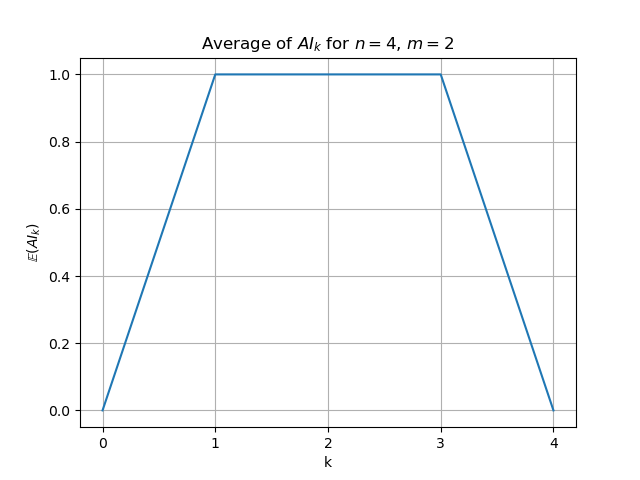
\includegraphics[width=\textwidth]{images/WPB_2_sample_size_full_dist.png}
        \caption{Mean $AI_k$}
        \label{fig:averagesFullDist}
    \end{minipage}
    \hfill
    \begin{minipage}[b]{0.5\textwidth}
        \centering
        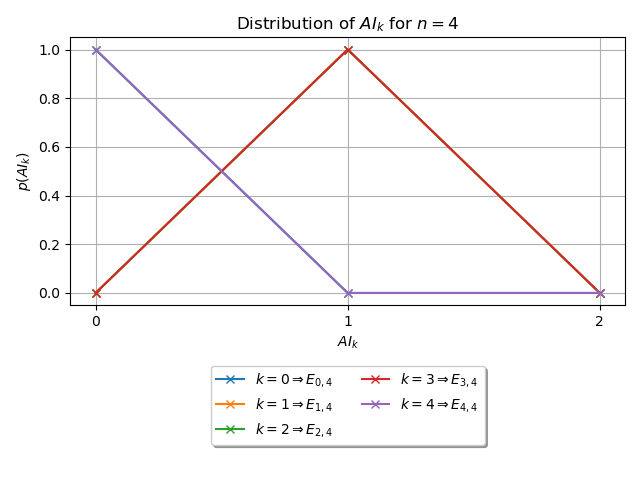
\includegraphics[width=\textwidth]{images/WPB_2_sample_size_full_dist_prob.png}
        \caption{Probability distribution of $AI_k$}
        \label{fig:probFullDist}
    \end{minipage}
    \caption{Mean $AI_k$ and probability distribution of $AI_k$ from Definition \ref{def:distAIk} of Boolean functions the family $WPB_2$ variable}
    \label{fig:dullDist}
\end{figure}


\begin{table}[ht]
    \centering
    \begin{minipage}{0.45\textwidth}
        \centering
       \begin{tabular}{rrr}
\toprule
 $k$ &  $AI_k(f)=d$ &  $p\left(AI_K(f) = d\right)$ \\
\midrule
   0 &            0 &                          1.0 \\
   0 &            1 &                          0.0 \\
   0 &            2 &                          0.0 \\
   \hline
   1 &            0 &                          0.0 \\
   1 &            1 &                          1.0 \\
   1 &            2 &                          0.0 \\
   \hline
   2 &            0 &                          0.0 \\
   2 &            1 &                          1.0 \\
   2 &            2 &                          0.0 \\
   \hline
   3 &            0 &                          0.0 \\
   3 &            1 &                          1.0 \\
   3 &            2 &                          0.0 \\
   \hline
   4 &            0 &                          1.0 \\
   4 &            1 &                          0.0 \\
   4 &            2 &                          0.0 \\
\bottomrule
\end{tabular}
        \caption{Probability distribution of $AI_k$ for $n=4$, $m=2$}
        \label{table:probFullDist}
    \end{minipage}\hfill
    \begin{minipage}{0.45\textwidth}
        \centering
        \begin{tabular}{rrr}
\toprule
 $k$ &  $\mathbb{E}[T(AI_k)]$ &  $\mathbb{E}[AI_k]$ \\
\midrule
   0 &               0.000038 &                 0.0 \\
   1 &               0.055785 &                 1.0 \\
   2 &               0.062083 &                 1.0 \\
   3 &               0.067631 &                 1.0 \\
   4 &               0.000105 &                 0.0 \\
\bottomrule
\end{tabular}
        \caption{Average execution time and $AI_k$ for $n=4$, $m=2$}
        \label{table:averagesFullDist}
    \end{minipage}
\end{table}

\subsubsection{Random Sampling}
In practice, the random sampling is done by generating a set $\Omega_k = \{\omega_1^{(k)}, \cdots, \omega_{|\Omega|}^{(k)}\}$ of $|\Omega|$ number of random balanced sub-truth tables for each slice $E_{k,n}$. Then, for each slice $E_{k,n}$ the $AI_k$ is calculated with each restricted set in $\Omega_k$ and a \textit{Montecarlo} is applied, counting the number of times a particular $AI_k$ is computed.\\
Depending on the value of $m$ and the chosen sample size, the number of sub-truth tables generated may be too large to fit in memory simultaneously. Therefore, it is essential to avoid storing all elements in memory at once. Instead, we should process them one by one, either by computing sequentially or by using iterators.\\ 

\pmnote{@Luca, what do you call a Montecarlo?}



The following procedure is done for each slice $E_{k,n}$.
\begin{enumerate}
    \item Initialize a hash table of all possible values of $AI_k$
    \item For each sub-truth table in $\omega_i^{(k)} \in \Omega_k$ ($\omega_i^{(k)}$ is either generated on the fly by an iterator or by having the source code for the generation of $\omega_i^{(k)}$ in this loop.)
    \begin{enumerate}
        \item Run Algorithm \ref{alg:fullAlg3ForAIRestrictesSetOpt} with $S=\omega_i^{(k)}$\label{enum:stepOfapplicationEnum}\\
        \item Increment the value in the hash table corresponding to the output of the previous step
    \end{enumerate}
    \item Divide each value in the hash table by $|\Omega|$.
\end{enumerate}

\textbf{Results for $n=8$ and sample size$=2^{15}$}\\
Figure \ref{fig:probDist32768} represent the $AI_K$ distribution and Figure \ref{fig:averages32768} $AI_k$ average values.\\
The table \lbnote{reference to table} shows the average values plotted in Figure \ref{fig:averages32768} and the average execution times and table \lbnote{Reference to table} shows the data of the probability distribution plotted in Figure \ref{fig:probDist32768}.

\begin{figure}[ht]
    \centering
    \begin{minipage}[b]{0.45\textwidth}
        \centering
        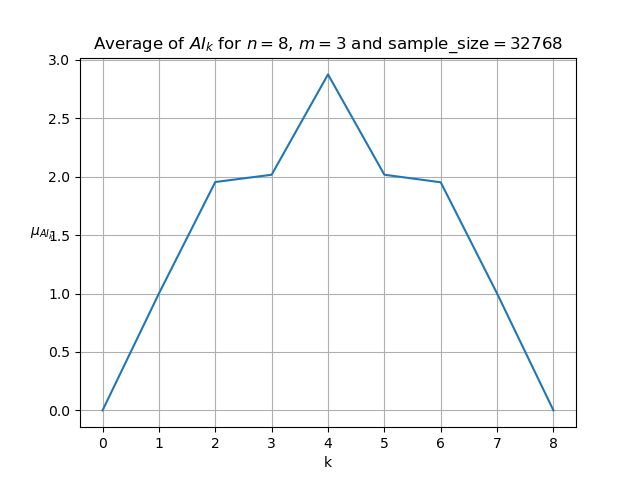
\includegraphics[width=\textwidth]{images/WPB_3_sample_size_32768_dist.png}
        \caption{Mean $AI_k$}
        \label{fig:averages32768}
    \end{minipage}
    \hfill
    \begin{minipage}[b]{0.5\textwidth}
        \centering
        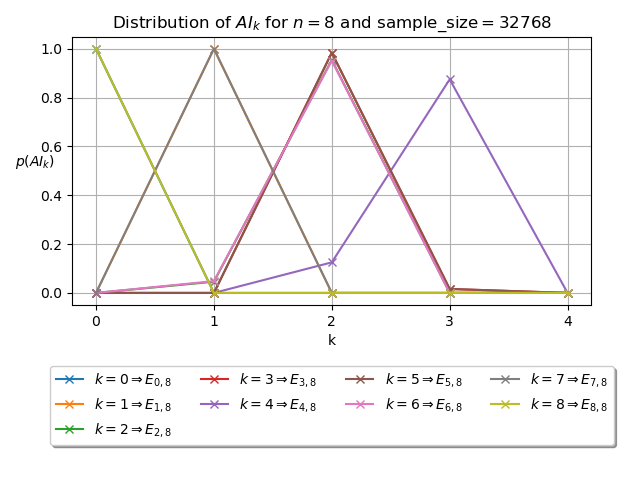
\includegraphics[width=\textwidth]{images/WPB_3_sample_size_32768_dist_prob.png}
        \caption{Probability distribution of $AI_k$}
        \label{fig:probDist32768}
    \end{minipage}
    \caption{Mean $AI_k$ and probability distribution of $AI_k$ with sampling size $23768$ of Boolean function of $n=8$ variable}
    \label{fig:main2}
\end{figure}


\section{Conclusion and open questions}

%\section{Acknowledgments}
%Pierrick Méaux was supported by the ERC Advanced Grant no. 787390.



\newpage

%%%%%%%%%%%%%%%%%%%%%%%%%%%%%%%%%%%%%%%~


\ifnum\full=0
%%%%%%%%%%%%%%%%%%%%%%%%%%%%%%%%%%%%%%%%%%%%
\bibliographystyle{splncs04}
\bibliography{add}
%%%%%%%%%%%%%%%%%%%%%%%%%%%%%%%%%%%%%%%%%%%%
\else
%%%%%%%%%%%%%%%%%%%%%%%%%%%%%%%%%%%%%%%%%%%%
\bibliographystyle{alpha}
\bibliography{add}
%%%%%%%%%%%%%%%%%%%%%%%%%%%%%%%%%%%%%%%%%%%%
\fi

%\newpage
%\appendix


\end{document}
